%%%%%%%%%%%%%%%%%%%%%%%%%%%%%%%%%%%%%%%%%%%%%%%%%%%%%%%%%%%%%%%%%%%%%%%%%%%%%%%%%%%%%%%%%%%%%%%%%%%%%%%%%%%%%%%
%%%%%%%%%%%%%%%%%%%%%%%%%%%%%%%%%%%%%%%%%%%%%%%%%%%%%%%%%%%%%%%%%%%%%%%%%%%%%%%%%%%%%%%%%%%%%%%%%%%%%%%%%%%%%%%
% Esta é apenas uma adaptação do ABNTex-2 para ser utilizado como tese ou dissertação de mestrado em inglês.
% Em resumo, os termos foram adptados para inglês (ex: Orietador se tornou Supervisor) e o modelo de citação, ao invés de 
% seguir um padrão todo maiusculo, foi trocado para minusculo (ex: FULANO; CICRANO; BELTRANO, 2010 se tornou Fulano, Cicrano, and Beltrano, % % 2010.
% Você pode se perguntar: Pra que usar o formato ABNT e inglês? Bom, algumas universidades não tem um padrão definido de tese/dissertação,
% e o ABNTex, com esses ajustes, fica um padrão bacana para ser seguido. Essas alterações visam poupar o seu tempo para configurar um projeto.
% Por fim, todos os créditos para a equipe que desenvolveu o pacote. Isso é apenas uma adaptação minuscula.
% Caso você venha a utilizar essa adptação, considere deixar a sua estrelinha para o projeto no Github, 
% isso valoriza e motiva desenvolvedores.
% Github: https://github.com/abntex/abntex2
% Faça bom uso!
% André Pacheco (pacheco.comp@gmail.com)
%%%%%%%%%%%%%%%%%%%%%%%%%%%%%%%%%%%%%%%%%%%%%%%%%%%%%%%%%%%%%%%%%%%%%%%%%%%%%%%%%%%%%%%%%%%%%%%%%%%%%%%%%%%%%%%
%%%%%%%%%%%%%%%%%%%%%%%%%%%%%%%%%%%%%%%%%%%%%%%%%%%%%%%%%%%%%%%%%%%%%%%%%%%%%%%%%%%%%%%%%%%%%%%%%%%%%%%%%%%%%%%

\documentclass[12pt, openright, oneside, a4paper, english]{abntex2}



%------------------------------------------------
%-------------- Pacotes necessários -------------
%------------------------------------------------

% Escrita 
\usepackage[T1]{fontenc}
\usepackage[utf8]{inputenc}
\usepackage{lmodern}
\usepackage{microtype} % para melhorias de justificação
\usepackage{indentfirst}

\renewcommand{\ABNTEXchapterfont}{\fontfamily{ptm}\fontseries{b}\selectfont}

% Gráficos 
\usepackage{color}
\usepackage{caption}
\usepackage{subcaption}
\usepackage{graphicx}
\usepackage{booktabs}  
\usepackage{multirow}               %for table
\usepackage{dcolumn}                %for decimal point align in table
\usepackage{siunitx}

% Matemáticos 
\usepackage{amsthm, amssymb, amsmath, mathtools}
\DeclareMathOperator*{\argmax}{arg\,max}
\usepackage[ruled,vlined, linesnumbered]{algorithm2e}

% Outros 
\usepackage{lipsum}

\usepackage[brazil]{babel}
\addto\captionsbrazil{%
\def\bibname{References}%
\renewcommand{\figurename}{Figure}
\renewcommand{\tablename}{Table}
\renewcommand{\listfigurename}{List of Figures}
\renewcommand{\listtablename}{List of Tables}
\renewcommand{\contentsname}{Contents}
\renewcommand\chaptername{Chapter}
}

\selectlanguage{english}


% ---
		
% ---
% Pacotes adicionais, usados apenas no âmbito do Modelo Canônico do abnteX2
% ---
\usepackage{lipsum}				% para geração de dummy text
% ---

% ---
% Pacotes de citações
% ---
%\usepackage{backref}	 % Paginas com as citações na bibl
%\usepackage[alf,abnt-and-type=&]{abntex2cite}	% Citações padrão ABNT
\usepackage[alf]{abntex2cite}	% Citações padrão ABNT


%\newtheorem{mydef}{Definição}[chapter]

%\usepackage{natbib}

% --- 
% CONFIGURAÇÕES DE PACOTES
% --- 

% ---
% Configurações do pacote backref
% Usado sem a opção hyperpageref de backref
%\renewcommand{\backrefpagesname}{Citado na(s) página(s):~}
% Texto padrão antes do número das páginas
%\renewcommand{\backref}{}
% Define os textos da citação
%\renewcommand*{\backrefalt}[4]{
%	\ifcase #1 %
%		Nenhuma citação no texto.%
%	\or
%		Citado na página #2.%
%	\else
%		Citado #1 vezes nas páginas #2.%
%	\fi}%
% ---

\newtheorem{name}{Printed output}

\selectlanguage{english}
\renewcommand{\orientadorname}{Supervisor}


% ---
% Informações de dados para CAPA e FOLHA DE ROSTO
% ---
\input{src/title-page}
\titulo{Events-Vis: A visual summary of spatio-temporal events that preserves areas and neighborhoods in a 2D plot}
\autor{Giovani de Almeida Valdrighi}
\local{Rio de Janeiro}
\data{2021}
\instituicao{%
  Getulio Vargas Foundation \\
  \par
  School of Applied Math
}
\tipotrabalho{Trabalho de Conclusão de Curso}

\preambulo{Final paper presented for the School of Applied Math (FGV/EMAp) as requirement for the undergraduate degree in Applied Math. \\ \\ Search area: visualization.}

\orientador{Jorge Poco}

% Se o seu texto tem subtítulo. 
% Se não tiver, altere o arquivo capa_folha_rosto_tex
%\subtitulo{}
% ---


% ---
% Configurações de aparência do PDF final

% alterando o aspecto da cor azul
\definecolor{blue}{RGB}{41,5,195}

% informações do PDF
\makeatletter
\hypersetup{
     	%pagebackref=true,
		pdftitle={\@title}, 
		pdfauthor={\@author},
    	pdfsubject={\imprimirpreambulo},
	    pdfcreator={LaTeX with abnTeX2},
		pdfkeywords={abnt}{latex}{abntex}{abntex2}{trabalho acadêmico}, 
		colorlinks=true,       		% false: boxed links; true: colored links
    	linkcolor=blue,          	% color of internal links
    	citecolor=blue,        		% color of links to bibliography
    	filecolor=magenta,      		% color of file links
		urlcolor=blue,
		bookmarksdepth=4
}
\makeatother

%-----------------------------------------------------
%--------------------- Margens -----------------------
%-----------------------------------------------------

\setlrmarginsandblock{3cm}{2cm}{*}
\setulmarginsandblock{3cm}{2cm}{*}
\checkandfixthelayout

%-----------------------------------------------------
%------ Espaçamentos entre linhas e parágrafos -------
%-----------------------------------------------------

% O tamanho do parágrafo é dado por:
\setlength{\parindent}{1.3cm}

% Controle do espaçamento entre um parágrafo e outro:
\setlength{\parskip}{0.2cm}  % tente também \onelineskip

% compila o índice
\makeindex

% ----
\begin{document}

% Retira espaço extra obsoleto entre as frases.
\frenchspacing 

% ----------------------------------------------------------
% ELEMENTOS PRÉ-TEXTUAIS
% ----------------------------------------------------------
\pretextual

% ---
% Capa
% ---
\imprimircapa
% ---
\cleardoublepage

% ---
% Folha de rosto
% (o * indica que haverá a ficha bibliográfica)
% ---
\imprimirfolhaderosto
% ---

% ---
% Inserir a ficha bibliografica
% ---
\input{src/ficha-catalografica}



% \begin{folhadeaprovacao}
%\begin{folhadeaprovacao}

    \begin{center}
      {\ABNTEXchapterfont\large\MakeUppercase{\imprimirautor}}
  
      \vspace*{\fill}\vspace*{\fill}
      \begin{center}
        \ABNTEXchapterfont\bfseries\large\MakeUppercase{\imprimirtitulo}	
      \end{center}
      \vspace*{\fill}
      
      \hfill
      \begin{minipage}{.7\textwidth}
          \imprimirpreambulo \\ \\
          And approved in 21/12/2021 \\
          By organizer comission
      \end{minipage}%
      \vspace*{\fill}
     \end{center}
  
     \assinatura{\imprimirorientador \\ School of Applied Math - FGV} 
     \assinatura{Nivan Ferreira \\ Centro de Informática - UFPE}
     \assinatura{Marcos Lage \\  Computer Science Institute - UFF}
     %\assinatura{\textbf{Professor} \\ Convidado 3}
     %\assinatura{\textbf{Professor} \\ Convidado 4}
\end{folhadeaprovacao}

% \begin{folhadeaprovacao}
% \includepdf{folhadeaprovacao_final.pdf}
% \end{folhadeaprovacao}


% ---
% Declaração de autoria
% ---
\newpage
\begin{center}
{\ABNTEXchapterfont\Large\textsc{Statement of Authorship}}
\end{center}
%
\vspace*{1cm}
%
I hereby declare that the thesis submitted is my own work. All direct or indirect
sources used are acknowledged as references. I further declare that I have not submitted
this thesis at any other institution in order to obtain a degree. %\\
%
% ---


%\newpage
% ---
% Dedicatória
% ---
%\begin{dedicatoria}
%  \vspace*{\fill}
%  \centering
%  \noindent
%  \textit{ To my friends and family. I am nothing without them.} \vspace*{\fill}
%\end{dedicatoria}
% ---



% ---
% Agradecimentos
% ---
%\begin{agradecimentos}
%
%I would like to thank all people from The Shire, in particular, my beloved nephew Frodo.
%
%\end{agradecimentos}
% ---

%\newpage
% ---
% Epígrafe
% ---
%\begin{epigrafe}
%    \vspace*{\fill}
%	
%	    \noindent
%		\textit{"One Ring to rule them all, One Ring to find them, One Ring to bring them all and in the darkness bind them.."}
%		
%		\begin{flushright}
%		J. R. R. Tolkien
%		\end{flushright}
%\end{epigrafe}


% ---
\newpage

 

 
\setlength{\absparsep}{18pt} 
\begin{resumo}[Resumo]
A análise de grupos em evolução no tempo é uma tarefa essencial no estudo de dados espaço-temporais.
Esses agrupamentos, geralmente detectados automaticamente, são utilizados para representar eventos  em muitas áreas, como mobilidade humana e surtos epidemiológicos.
%
A realização de análises visuais desse tipo de dados é um desafio para as técnicas recentes devido a fatores como extensão espacial, interseções espaciais e evolução temporal.
%
Tudo isso faz com que as técnicas baseadas em mapas amplamente utilizadas sofram de excesso de primitivas gráficas e oclusões, portanto, ineficazes para este propósito.
%
Já as técnicas de visualização que usam animação ou interatividade para representar as três dimensões, apresentam limitações de interpretação.
%
Para superar essas limitações, apresentamos  Events-Vis, um método para visualizar dados de eventos espaço-temporais em um gráfico temporal estático, representando o espaço em uma dimensão. Linearizamos o espaço usando duas estratégias: um algoritmo guloso e uma otimização convexa. Em ambos os casos, nosso objetivo é preservar vizinhanças e intersecções.
%
Demonstramos a eficácia do nosso método em uma série de experimentos e um estudo de caso usando conjuntos de dados sintéticos e do mundo real.

 Palavras-chave: visualização, espaço-temporal, agrupamento
\end{resumo}

% resumo em português
\setlength{\absparsep}{18pt} % ajusta o espaçamento dos parágrafos do resumo
\begin{resumo}[Abstract]
 \begin{otherlanguage*}{english}


The analysis of time-evolving clusters is an essential task in the study of spatio-temporal data.
People often use these clusters to represent events automatically detected in many fields, such as human mobility and disease outbreaks.
%
Performing visual analysis of this data type is challenging for current state-of-the-art techniques due to factors such as spatial span covered by clusters, spatiotemporal intersections, and temporal evolution.
%
All of this makes widely used geographical map-based techniques suffer from overplotting and cluttering, therefore, ineffective for this purpose.
%
Visualization techniques used to analyze results use animation or interactivity to represent the three dimensions, but they show limitations on interpretation.
%
To overcome these limitations, we present Events-Vis, a method for visualizing spatio-temporal clusters event data in a static temporal plot by representing the space in one dimension. We linearize the space using two strategies: a greedy algorithm and a convex optimization. In both cases, our goal is to preserve neighborhoods and intersections. 
%
We demonstrate the effectiveness of our method in a series of experiments and a case study using both synthetic and real-world datasets.


\textbf{Keywords:} Visualization, spatiotemporal, clustering

\end{otherlanguage*}
\end{resumo}

\newpage


% ---
% inserir lista de ilustrações
% ---
\pdfbookmark[0]{\listfigurename}{lof}
\listoffigures*
\cleardoublepage
% ---

% ---
% inserir lista de tabelas
% ---
\pdfbookmark[0]{\listtablename}{lot}
\listoftables*
\cleardoublepage
% ---
%\begin{siglas}
  %\item[MSE] Erro médio quadrático
  %\item[FLR] Relacionamento Lógico Fuzzy
%\end{siglas}

% ---
% inserir o sumario
% ---
\pdfbookmark[0]{\contentsname}{toc}
\tableofcontents*
\cleardoublepage
% ---

% ----------------------------------------------------------
% ELEMENTOS TEXTUAIS
% ----------------------------------------------------------
\textual

% ----------------------------------------------------------
% Introdução (exemplo de capítulo sem numeração, mas presente no Sumário)
% ----------------------------------------------------------
\chapter{Introduction}
The increase in the use of GPS devices on cars, smartphones, and remote sensors permitted the collection of information about the spatial distribution of entities,
%
as this data is collected constantly, the time information of measurements is an important aspect of it.
%
\textit{"Spatio-temporal"} refers to the data with both spatial and temporal information, and it can be of different types.
%
Different methods of data mining are used to obtain the most important characteristics to analyze the data~\cite{ansari2020spatiotemporal}, and one of the most common is clustering techniques.
%
By creating clusters, the data is separated into groups that relate to real events in the observed system, and it is used in many domains such as human mobility, healthcare, seismology, and climate science~\cite{BELHADI2020103857}. 
%

While these techniques help analysts reveal possible patterns, the spatio-temporal nature and complexity of these clusters make their visual representation challenging. 
%
The results will have at least three dimensions, one temporal and two spatial, and may have more information such as categories, labels, requiring techniques to view multivariate data. 
%
This problem makes widely used geographic map-based techniques suffer from over-plotting. 
%
Space-time Cube, animations, and small-multiples are some of the used methods for spatio-temporal visualization, although, they present some problems of cluttering, overplotting, and cognitive limitations. 

To overcome these limitations, it was developed Events-Vis, a method for the visualization of spatio-temporal events that seek to represent this three-dimensional information in a static temporal plot.
%
Focusing on the preservation of areas and neighborhoods of events, we visually approximate the 2D spatial context into a 1D axis by using dimensionality reduction and optimization techniques. 

The organization of this document is: on Section~\ref{ch:background} is presented the already done work in spatio-temporal visualization and a description of projection methods and clustering (to create events), on Section~\ref{ch:methodology} is presented the development of this work, the details of the created visualization technique, the implementation of a web visualization tool and the description of how the method was evaluated, on the last Section~\ref{ch:results} is shown the results obtained from the visualization, presenting the evaluation of the method and a use case on real-world data.

The implementation of the proposed method, with the web interfaces, the data and the experiments are available publicly at~\cite{Giovani2021}.

\chapter{Background}
\label{ch:background}

A theoretical background is now presented, we first look at the methods of spatio-temporal visualization, and after that focus on two transformations that are going to be used on the proposed method, the dimensionality reduction and the clustering of points.

\section{Spatio-temporal visualization}

Map visualization has been used for more than centuries and has an extensive search done.
%
Recently, with the increase of spatio-temporal data, the most used methods for visualization uses the techniques from cartography to represent spatial information and the dynamic aspect of computer-based visualizations to represent time: interactivity and animations. 
%
To present an overview of the spatio-temporal visualizations already made, we will talk about widely used techniques and recent works that inspire and relate to Events-Vis.

\subsection{Space-time cube}

The Space-Time Cube, as the name says, is a plot created with the use of a three-dimensional cube such that the base represents the 2D space and the height represents the time dimension~\cite{bach2017descriptive}.
%
With that formulation, the STC is a very general method and supports different graphic primitives to represent different types of data and different types of attributes, such as trajectories, events, with categorical or numerical attributes.
%

Figure~\ref{fig:space-time-cube-reference} is shown the use of a STC for a trajectory, on the base of the cube is drawn a map of the city that the data is from, and a black line is marked linking the points of the personal travel during the day, as the black line increases in the height, it indicates the passing time. On the visualization are some marks to increase the interpretability, and for example, it is possible to check that the person left the house at 05:10 and returned at 19:55.

\begin{figure}
    \centering
    \includegraphics[width = 0.7\textwidth]{src/imgs/space-time-cube-reference.png}
    \caption{Source: \cite{Kraak2003Space}. Space-Time Cube visualization of a trajectory of a routine day of a person in a city.}
    \label{fig:space-time-cube-reference}
\end{figure}
%
Many visualizations use the STC linked to other views to permit better analyses of the data with other attributes than the spatio-temporal information.
%
However, as the cube is a 3D object represented in a 2D screen of a computer, it is necessary a projection that can lead to bad positioning of the graphic primitives, causing cluttering and distortion of space and time~\cite{andrienko2013visual}.
%
In the example in Fig.~\ref{fig:space-time-cube-reference}, it is not totally possible to compare the distance between \textit{pool} and \textit{work}, and the distance between \textit{work} and \textit{restaurant} due to the projection of the 3D cube.

\subsection{Small-multiples}

Small-multiples is a visualization method that uses sequential map plots to represent the time evolution of the data, the total time interval is divided into smaller periods and the data from each period is plotted in a separated map.
%
This method permits the flexibility to use any map visualization that do not consider the time, and just create it for different fixed time intervals.
%
In Figure~\ref{fig:small-multiples-reference} is presented a small multiple visualization of the progress of approved land for harvesting in the Hood Canal. 
%
Each of the individual eleven maps represents a year of the data and uses coloring in each to mark the approved areas.

\begin{figure}
    \centering
    \includegraphics[width = \textwidth]{src/imgs/small-multiples-reference.jpg}
    \caption{Source: \cite{peterson2011small}. A yearly time-series of the approved lands for harvesting in on Hood Canal plotted with a small multiples visualization.}
    \label{fig:small-multiples-reference}
\end{figure}

However, a limitation to the method is the number of views that can be represented on the screen, as the number can not get big, and that it is not simple to identify the best detail to discretize time and generate the multiple views~\cite{Andrienko2003exploratory}.
%
As shown in the example, the  maps take a big screen size and are limited to an interval of eleven years.

\subsection{Animations}

Animations can be used in any form of visualization, it permits to update the figure with new information and can lead the attention of the viewer.
%
On spatio-temporal data, basic map plots are created to represent the 2D space and the time is represented by the physical time, i.e., the pass of the time in the data is represented with the pass of the real-time.
%
To increase the quality of the visualization, the user can select intervals where they want to visualize the animation, jumps between timestamps, control the velocity.
%

However, even with this flexibility of control, animations visualization suffers from a cognitive limitation.
%
To compare data from different timestamps, the user needs to memorize the figure as it is not possible to visualize them simultaneously, and as already known, the human brain can keep track of only a small number of changing objects~\cite{Harrower:2007:Cognitive}. 
%
\subsection{Recent methods}
%
With most visualization tools proposed for spatio-temporal data using linked views and interactivity, some recent methods have been using static 2D plots to represent an overview of the data.
%
The idea is to represent the space as a function of time, and as usual, the time is represented in the horizontal.
%
With that, the 2D space is represented in a 1D vertical axis and a projection method is necessary to make this space transformation.

With minor changes according to the objective, some of the examples of this method are: \cite{Buchmuller:2018:MVCTST}, \cite{spatialrugs}, \cite{wulms2021stable} and \cite{1dordering}.

\begin{figure}
    \centering
    \includegraphics[width = \textwidth]{src/imgs/motionrugs.png}
    \caption{Source: \cite{Buchmuller:2018:MVCTST}. Pipeline of the MotionRugs visualization technique, the data used is the movement of a set of fish in an aquarium.}
    \label{fig:motionrugs}
\end{figure}

In Fig.~\ref{fig:motionrugs} is presented an example of the method MotionRugs and the process of generating the visualization.
%
Each time frame is represented as a column, the column is filled with pixels, one for each object in the space, that are ordered based on a projection method.
%
In the example, it is a visualization generated from a set of fish moving in circles in an aquarium, each pixel in the column is a fish. 
%
The beautiful result of the visualization is obtained with the coloring based on the velocity of each fish.
%
With this view, it is possible to observe the general movement of observed entities, comparing different timestamps without occlusion or distortions.

%
As the objective of the method is to visualize collective moments, it only considers the relative position between objects and only permits the interpretation of the group trend of movement.
%
Besides that, it is limited to trajectories of objects that are observed in the complete period, so in the scenario of spatio-temporal events with small periods of occurrence, there is not a simple adaptation.

\section{Space transformation}
\label{seq:space-transformation}

As previously mentioned, many proposed visualizations for spatio-temporal data uses an axis to represent the spatial distribution of data,
%
with the use of space transformation methods to represent the information contained in 2 dimensions in a 1D axis.
%
The transformation of space is a very common task in many domains with different properties depending on the objectives of the representation.

%
In this section will be presented a general overview of space transformation methods, 
%
separating in methods for dimensionality reduction of high-dimensional data and methods of spatial indexing that are heavily used in computer science.
%
A brief example of the different projection methods is presented in Fig.~\ref{fig:projection-example} on a dataset with two variables.

\begin{figure}
    \centering
    \includegraphics[width = \textwidth]{src/imgs/projection-example.pdf}
    \caption{Source: elaborated by author. Considered projection methods in an example dataset. The ordering of points is represented by the line connecting them, each point is connected to its predecessor and successor.}
    \label{fig:projection-example}
\end{figure}

\subsection{Dimensionality reduction}
%

With the recent advancements in technologies and means of communication, the availability, of high-dimensional data increased exponentially. 
%
Despite it great value of information, machine learning methods and algorithms can suffer from dimensionality problems.
%
Methods to represent the valuable information in lower dimensions have been developed and are vastly used.
%

Based on the overview presented by~\cite{ayesha2020dimensionality}, dimensionality reduction techniques are methods that transform high-dimensional data $Y = [y_1, \dots, y_m] \in \mathbb{R}^{m \times p}$ with dimension $p$ and $m$ samples to a new data in low dimensionality $Z = [z_1, \dots, z_m] \in \mathbb{R}^{k \times m}$ keeping the same $m$ samples but in a lower dimension, generally $k << p$. 
%

In this subsection will be presented the methods PCA, MDS, UMAP, and t-SNE.

\subsubsection{Principal Components Analysis}
%
PCA was first introduced by Pearson in 1901 and is one of the most studied methods of dimensionality reduction, and with many adaptations for different applications~\cite{ayesha2020dimensionality}.
%
The idea is that with p-dimensional data, there are dimensions that are of less interest when identifying different observations, so it is possible to reduce this dimensionality by maintaining only the dimensions with the greatest variance.
%
However, PCA is not a method for the selection of the features, what it does is to create new dimensions from a linear combination of the original $p$ dimensions, each of these created dimensions is called a \textit{principal component}.
%

With the same notation $Y\in \mathbb{R}^{m\times p}$, and $y_i \in \mathbb{R}^m, \forall i \in \{ 1, \dots, p\}$ the columns of $Y$, the first principal component is defined as~\cite{james2013introduction}:

\begin{equation*}
\begin{split}
    z_1 = \begin{cases}
    \argmax Var(z) \\
    z = \theta_{11}y_1 + \theta_{21}y_2 + \dots + \theta_{p1}y_p \\
    \sum_{i=1}^p\theta_{i1}^2 = 1
    \end{cases}
\end{split}
\end{equation*}

With $\theta_{1} = (\theta_{11}, \dots, \theta_{p1}) \in \mathbb{R}^p$ called \textit{loading}.
%
We can define the second principal component $z_2$ in a similar manner, a linear combination of $y_i$ that maximizes the variance, with normalized loading and with the additional constraint that $z_1$ and $z_2$ must be uncorrelated. 
%
Following $m = \min{(n -1 , p)}$ principal components can be defined in the same manner.
%

%
To apply PCA for space transformation, we generate a low dimensional $k$ representation of $Y$ in dimension $p$ by computing the first $k$ principal components and building a matrix with the components as columns $Z = [z_1, \dots, z_k]$, $z \in \mathbb{R}^{m\times k}$.
%
There are different manners to compute the loadings $\theta_i$ and following components, the most common being by using the eigenvectors from the covariance matrix of $Y$. 

\subsubsection{Multidimensional scaling}
%
MDS is a method similar to PCA, but the main difference is that instead of working with points in $\mathbb{R}^p$, 
%
MDS uses dissimilarity measures between pairs of points and tries to recreate a representation in a space of any dimension, generally low dimension, with the distances between points equal to the original dissimilarity measure.
%
The origin of this dissimilarity measure is not important for the method and can be any distance metric such as euclidean distance, Manhattan distance, or any other, per example, to obtain a 2D representation of the distance between cities of a country, it can be used the time necessary to travel by train between cities as a dissimilarity measure.
%
This presentation is based on the work from \cite{cox2008multidimensional}.
%

There are different versions of MDS, the most common are metric (or classical) and non-metric. 
%
Let $d_{i, j}$ be the dissimilarity measure between objects $i$ and $j$.
%
In the metric version, $d_{i, j}$ is interpreted as a distance value, although,
%
in the non-metric version, it is considered that $d_{i, j}$ does not fully represent a distance, and only the rank order of the value is used, i.e., the point farther from $i$ in the original space will be the farther in the calculated representation of $i$.
%

For a set of $m$ objects, with values $d_{i, j}$ defined above, a projection using MDS is a set of $m$ points in $\mathbb{R}^{p}$, usually with $p \in \{2, 3\}$, such that the euclidean distance between points $\hat d_{i, j}$ is close to $d_{i, j}$.
%
A metric to evaluate the goodness-of-fit is the stress measure defined as:

\begin{equation}
    S = \sqrt{\dfrac{\sum_{i = 1}^m \sum_{j = i + 1} ^m (d_{i, j} - \hat d_{i, j})^2}{\sum_{i = 1}^m \sum_{j = i + 1}^m  d_{i, j}}}
\end{equation}
\label{eq:stress-measure}

We have that $S \in [0, 1]$, and $S = 0$ means perfect representation and $S$ nears to $1$ means poor fitness.


%
To calculate the points, metric MDS apply a transformation in the matrix $D$ of dissimilarities and after uses the decomposition in eigenvalues and eigenvectors, similar to PCA. 
%
The non-metric version applies optimization algorithms in the stress metric.

\subsubsection{t-Distributed Stochastic Neighbor Embedding}
%
t-SNE~\cite{van2008visualizing} is one of the most used methods for visualizing high-dimensional data 
%
and compared with the other two mentioned methods,
%
it is a more advanced technique that creates probabilities of connections between points in the high-space and 
%
represents it in a low-space using the t-Student distribution.
%
We now present a general overview based on the great explanation in~\cite{stelling2019entendendo}.
%

Initially, with values $Y$ in high-space, the distance between points is computed and transformed to a probability using the Gaussian distribution.
%
This transformation uses a variance value for each point, this value is determined with the hyper-parameter called \textit{perplexity}. 
%
To obtain the representation on low space, a t-Student distribution is used to approximate the samples in the high dimensional space, the measuring of the divergence between the two distributions is the KL-Divergence.

With the parameter \textit{perplexity}, the t-SNE projection method can variate in the preservation of local structure or a global structure, however, there is the need to fit this parameter according to the dataset and the desired result.
%
Due to its complexity, the method also presents a longer computing time than the previous methods.

\begin{figure}
    \centering
    \includegraphics[width = \textwidth]{src/imgs/umap-explanation.png}
    \caption{Source: \cite{sainburg2021parametric}. UMAP dimensionality reduction process. The \textit{non-parametric} method is the method described in this work.}
    \label{fig:umap_explanation}
\end{figure}

\subsubsection{Uniform Manifold Approximation and Projection}
%
UMAP is a recent method from~\cite{mcinnes2020umap} that competes with t-SNE the status of state of art in dimensionality reduction.
%
The presentation of the method will be based on the introduction made in~\cite{coenen2018umap}.
%

The process of space transforming from UMAP can be divided into two steps as shown in Figure~\ref{fig:umap_explanation}: the creation of a graph with the high-dimensional data, and the representation of this graph in low-dimension. 
%
In the example, 3D data is transformed to be plotted in 2D.
%
The graph is formed from the data points as vertices, and the weighted edge between two vertices indicates the connectedness of the points.
%
To construct this graph, from each point a radius is drawn, 
%
other points inside this radius are considered connected to the initial point,
%
the length is this radius must be adequate to avoid isolated points and avoid connect all points.
%
For that reason, it is based on the distance between the point and its $n$-th nearest neighbor.
%
Points that are inside this radius and closer to the initial point will have edges with bigger weights than points that are also inside the radius, but farther from the center.
%
After this graph is built in high-space, an optimization process is used to generate a similar layout of points in a low-dimensional space.
%

The two parameters that affect the projection obtained from UMAP are the \textit{number of neighbors} and the \textit{minimum distance}.
%
As already mentioned above, the number of neighbors is used in constructing the graph in high-dimension, 
%
when the number of neighbors considered is high, more connections between points will be created, and the graph will represent more the global structure of the data,
%
when it is low, the method will give more importance to local patterns of the data, as only really close points will be connected.
%
The other parameter is used in the construction of the low-dimensional representation, it is the minimum distance between two points in the new space,
%
when its value is low, points will be close together,
%
when it is high, points will have more freedom to arrange themselves but can lead to noisy results.
%

UMAP presents really good results in different patterns of high-dimensional data.
%
However, due to having two parameters,
%
to obtain good results for a specific dataset is necessary to try different combinations of parameters and analyze the different results.
%

\subsection{Spatial indexing}

As defined by~\cite{azri2013review}, spatial indexing is a technique to optimize query processing in large spatial databases,
%
it organizes rows of information on memory in such a manner that search is efficient.
%
The use of spatial indexing methods for projection is because to make faster queries,
%
the structures built need to preserve proximity between points, 
%
creating a good representation of the space that can be traversed to get a 1D projection.
%
It can be divided into two categories, space driven structures, that are dependent only on the space of the data, 
%
and data-driven structures, that depending on the points used, will generate different structures.
%
Examples of space-driven structures are trees such as Quadtree and KD-Tree, and space-filling curves that will be presented in this work.
%

With the proof of George Cantor that the interval $[0, 1]$ can be mapped bijectively to the unit square $[0, 1] \times [0, 1]$ in 1878, 
%
the discussion if this map could be continuous started, with the following result by E. Netto that if the map is bijective, it is necessarily discontinuous. The remaining question was if there could be a surjective and continuous map.
%
In 1890 Giuseppe Peano answered this question by constructing a function that had this property~\cite{sagan2012space}.

%
Now called space-filling curves, they are functions $f : [0, 1] \to [0, 1]^2$ that for each $(x, y) \in [0, 1]^2$, there is $z \in [0, 1]$ such that $f(z) = (x, y)$.
%
They are generally defined by a limit of functions that are not surjective in the unit square, but when the limit is applied, it can be shown that is convergent and the resulting function is space-filling.

%
In this text, we will focus on the geometric interpretation of space-filling curves. They can be generated by a process that is recursive and self-similar, exemplified in Figures~\ref{fig:hilbert-curve} and \ref{fig:morton-curve}.
%
Although not being one of the objectives when were created, these curves present a property that close points in the interval will be mapped to neighborhoods in the unit square, a characteristic that is highly useful in computational sciences to build data structures (spatial indexing) or in algorithms \cite{bader2012space}.

\subsubsection{Hilbert curve}

Hilbert-curve is a space-filling curve proposed by David Hilbert in 1891 \cite{Hubert1891}. The curves of order from 1 to 6 can be seen in Fig.~\ref{fig:hilbert-curve}.
%
The iterative process of creating the Hilbert curve starts by dividing the unite square into four smaller squares, as shown in the curve of order 1,
%
then these squares are traversed by following a format of an upside-down \textit{U},
%
the green line represents the curve of order 1.
%
To get the curve of order 2, each of the four smaller squares from the previous curve is divided again into 4 equal parts.
%
In each of them, a curve of order 1 is placed, 
%
in the image there are two copies in color green exhibited,
%
the other two copies are not so easily identified because they are rotated to connect with the remaining of the line without self-crossing.
%
The curves of bigger order are created in the same manner: dividing each square in 4, and connecting 4 copies of the curve of the previous order, two in the same orientation and two rotated.
%
In the figure, there are indications of one of the copies for curves of orders 3 and 4.
%

To obtain a projection of data $Y \in \mathbb{R}^{m \times 2}$, the first step is to move the data to the unit-square, 
%
this can be done by just subtracting the minimum and dividing by the range in each of the two dimensions.
%
Now the curve is traversed, by determining a start point (on the figure, the bottom left),
%
and walking through the unit square, each of the smaller squares is numbered by the order of passing.
%
In the example of the curve of order 1, the square $[0, 0.25]^2$ receives the number 1 because of being the first visited,
%
the square $[0, 0.25] \times [0.25, 0.5]$ is the second visited and receives the number 2.
%
In the image, there are some examples of numbering for curves of orders 2 and 3.
%
For the data points, the projection value is the number of the square that is contained.
%

The projected data $Z$ will be discrete, i.e., $z_i \in \mathbb{Z}$, and with the order of the curve being $k$, the maximum value obtained will be $4^k$. 
%
Depending on the application, these projection values can be divided for $4^k$, obtaining that $z_i \in [0, 1]$.


\begin{figure}
    \centering
    \includegraphics[width = \linewidth]{src/imgs/hilbert-curve.pdf}
    \caption{Source: Braindrain0000, CC BY-SA 3.0 \url{<http://creativecommons.org/licenses/by-sa/3.0/>}, via Wikimedia Commons, adapted by the author. Hilbert curves of a different order, the numbers beside the curves indicate the projected value represented by the square, and the change of colors in the same curve highlight the shape of the curve of the previous order.}
    \label{fig:hilbert-curve}
\end{figure}

\begin{figure}
    \centering
    \includegraphics[width = 0.5\linewidth]{src/imgs/morton-curve.pdf}
    \caption{Source: Public domain, adapted by the author. Morton curve of order 3, on the top left corner, a curve of order 2 is built with 4 copies of the curve of order 1 that are colored with blue..}
    \label{fig:morton-curve}
\end{figure}

\subsubsection{Morton curve} 

The Morton curve, shown in Figure~\ref{fig:morton-curve}, is very similar to the Hilbert curve, with the same process of generation, by dividing in 4 and replicating previous curves.
%
Despite, the curve of order 1 does not have the upside-down \textit{U} shape, it has a \textit{Z} shape, and for that reason is commonly called of Z-Order curve.
%
Another difference is that the copies of the curve are not rotated.
%
In the Figure, the 4 copies of the curve of order 1 that are used to create the curve of order 2 are marked with blue color.

A projection can be made with the Morton curve with the same process described to project with the Hilbert curve.
%

Many other space-filling curves exist and are used for spatial-indexing, although,
%
the present work will only consider the Hilbert and Morton curve due to the big number of already considered projection methods 
%
and their prevalence in applications.

\section{Clustering}
\label{sec:clustering}

Clustering is a very common unsupervised method for data mining \cite{ansari2020spatiotemporal}, the objective is to separate data points in groups that are similar and, in some cases, noise points.
%
In the context of spatio-temporal data, there is the necessity of the adaptation of methods due to the different nature of distance in the spatial and temporal dimensions. 
%
While time is 1D, the space is 2D, and there is no simple relation between our measurements of time (seconds, hours, days) and our measurements of space (meter, kilometer, degree), so when searching for neighborhoods, these two subsets of the attributes of the data must be handled differently.
%
Adapted methods were already proposed and \cite{ansari2020spatiotemporal} present a review of them.
%
In this section, it is presented the method ST-DBSCAN, a variation of the method DBSCAN~\cite{ester1996density} for spatio-temporal data, and was used in this work to identify events.
%

\subsection{DBSCAN}
DBSCAN was proposed by \cite{ester1996density} and still today one of the most used methods, with many adaptations, improvements, and experimentation.
%
The idea is that a cluster of points presents a higher density inside than outside of it, and that this density is related to the number of neighbors of each point. Some definitions from the original article will now be presented:
%

\textbf{Neighborhood of a point} For a set of points $D$, a point $p$ and distance function $d$, the neighborhood of $p$ with threshold $Eps$ is $N_{Eps}(p) = \{ q | d(p, q) \leq Eps, q \in D \}$. The sub index of $N_{Eps}(p)$ will be omitted.
%

\textbf{Directly density-reachable} A point $p$ is directly density-reachable from $q$ if $p \in N(q)$ and $N(q) \geq MinPts$.
%

\textbf{Density-reachable} A point $p$ is density-reachable from a $q$ if there is a sequence of points $p, p_1, \dots, p_k, q$ such that consecutive points are directly density-reachable.
%

\textbf{Density-connected} Two points $r$ and $s$ are density-connected if there is a point $p$ such that both are density-reachable to $p$.
%

The intention of the previous definition was to construct the idea of a cluster.  
%
Points from the same neighborhood would be included in the same cluster, but it is a restrict constraint, so points that density-reachable will also be considered in the same cluster, and as it is difficult to happen between border points, points density-connected are also considered to be in the same cluster.
%

\textbf{Cluster} Let $D$ be a database of points, a cluster $C$ with thresholds $Eps$ and $MinPts$ is a non-empty subset of $D$ if:
\begin{itemize}
    \item $\forall p, q \in D$ if $p$ is density reachable from $q$ and and $p \in C \implies q \in C$.
    \item $\forall p, q \in C$, $p$ and $q$ are density-connected.
\end{itemize}
%

To compute clusters according to the previous definition, the algorithm iterates over points, calculating the neighborhood and verifying if the number of points is bigger than $MinPts$, then each point of the neighborhood is added to a stack, and for each point $q$ in the stack, the neighborhood is calculated and the size verified, if it is bigger than $MinPts$, all points are added to the stack, and this process repeats until the stack is emptied.

\subsection{ST-DBSCAN}

The now presented method ST-DBSCAN~\cite{BIRANT2007208} improves DBSCAN by initially considering two thresholds $Eps_1, Eps_2$ for the neighborhood, with $Eps_1$ being the threshold for the spatial variables and $Eps_2$ the threshold for time variables. Another adaptation is the addition of a parameter $\Delta \varepsilon$ that limits the search for density-reachable points, the distance between the mean of non-spatial attributes of points from a cluster $C$ and a new point $q$ should be smaller than $\Delta \varepsilon$ to be considered the same cluster. The algorithm is present in \ref{alg:dbscan}.

\begin{algorithm}[H]
\label{alg:dbscan}
\SetAlgoLined
\SetKwInOut{Input}{Input}
\Input{
$D$ - set of objects \\
$Eps_1$ - threshold for spatial distance in neighborhood \\
$Eps_2$ - threshold for temporal distance in neighborhood \\
$MinPts$ - threshold for the number of points to consider a cluster \\
$\Delta \varepsilon$ - threshold to verify when adding to cluster 
}
\SetKwInOut{Output}{Output}
\Output{
$C$ - array with cluster id for each point, value $-1$ for noise points
}
cluster\_label $= 0$ \;
\For{$p \in D$}{
\If{$p$ not in a cluster}{
$N = $ retrieve\_neighbors$(p, Eps_1, Eps_2)$\;
\uIf{$|N| < MinPts$}{
Mark $p$ as noise \;
}
\uElse{
cluster\_label++\;
\For{$q \in N$}{
Mark $q$ as cluster\_label\;
}
stack $= N$\;
\While{stack is not empty}{
q = stack.pop()\;
$N_q =$ retrieve\_neighbors$(q, Eps_1, Eps_2)$\;
\If{$|N_q| >= MinPts$}{
\For{$s \in N_q$}{
\If{($s$ not in a cluster) 
and (distance\_cluster\_center$(s) \leq \Delta \varepsilon$) }{
Mark $s$ as cluster\_label\;
stack.add($s$)\;
}
}
}
}
}
}
}
\caption{ST-DBSCAN}
\end{algorithm}



\chapter{Methodology}
\label{ch:methodology}

\section{Development}

The main goal of this work is to present a novel technique for visualizing events with space and time information but keeping most of this 3D distribution (i.e., longitude, latitude, and time) in a 2D plot.
%

Inspired by the work done in MotionRugs~\cite{Buchmuller2019} and from Max Franke et.al.~\cite{franke2021visual} in spatio-temporal visualization where it is created a heatmap with the time in one axis and the bi-dimensional space represented in the other, 
%
it was desired to develop a method with this characteristic that was able to represent events and their areas, intersections areas, and that were not observed the complete time period.


\section{Events-Vis: Method}

%
The initial adaptation was to transform the heatmap used in the literature into a scatter plot,
%
so it was possible to represent events as rectangles with different widths and heights, instead of fixed grid size, and use these two properties to represent data features.
%
In the scatter plot, time will be mapped to the horizontal axis, and the width of rectangles will represent the temporal size of events; space will be mapped to the vertical axis, with the height of rectangles representing the area of the region of the event.
%

The horizontal axis can be easily created with a linear scale based on the time information of start and end of events, so the width would be representing the duration of an event. 
%
To create the vertical axis, it was necessary to transform the 2D information to 1D, and differently from the literature, a projection could not be applied directly to events because they are not single points.
%
A solution to this task was a development of a method for vertical positioning that initially uses a projection, and after that try to adjust for the intersection between events.

\begin{figure}[th]
    \centering
    \includegraphics[width = \textwidth]{src/imgs/pipeline.pdf}
    \caption{Source: elaborated by author. Events-Vis pipeline: 1) events are initially ordered, 2) based on this ordering, on the area, and area of intersections, the rectangles are positioned vertically, 3) the inner structure of rectangles is represented inside each one.}
    \label{fig:pipeline}
\end{figure}

The pipeline of this method is exhibited in Figure~\ref{fig:pipeline}, and can be divided into three steps: 1) the center position of events is computed and events are ordered based on a projection, 2) the rectangles representing events are positioned vertically and 3) the inner points of each event are represented inside rectangles. Each step will be detailed in the following sections.

\textbf{Algorithm input} Consider that we have a set of $n$ events denoted by $(e_i)|_{i = 1}^n$, if events are composed by a set of points, it can be computed a convex hull to represent the spatial span of points, otherwise, events must also include information of a polygon in space. 
%
For each, there is a measure of area of the spatial span $a_i \in \mathbb{R}^+$, for each pair of events $(e_i, e_j)$ there is also a measure of the area of spatial intersection $w_{i, j} \in \mathbb{R}^+$.

\subsection{Events Ordering}

To project events from 2D to 1D it is possible to use a point as a representative of each event, and project this point to obtain a projection of events. 
%
The representative point can be the mean of points if there is a set of points or can be the mass center of the spatial shape of the event.
%
From this projection, it is obtained an ordering of events, if the projection of $e_i$ was smaller than the projection of $e_j$, it will denote that $e_i < e_j$.
%
On Figure~\ref{fig:pipeline} a) there are example events and the respective convex hulls, that have their center projected on b), obtaining the exhibited order.

%
The projection methods used were the methods described in section \ref{seq:space-transformation},
%
the result of the visualization is highly dependent on the choice of projection method, so it is necessary an evaluation of the considered methods.
 
\subsection{Vertical Positioning}

In the second step, the order of events will be used to position the rectangles on the vertical axis. 
%
As the horizontal direction represents time, in this step the rectangles can be simplified to segments perpendicular to the x-axis, $s_i$ being the segment of event $e_i$. Consider that the index of events is based on their order, i.e., if $i < j$  the order of events obtained in the projection step is $e_i < e_j$. 
%

%
Let $(0, y_i)$ be the mean point of segment $s_i$ in the Cartesian plane and $h_i$ be its length, i.e., the segment $s_i$ starts at the point $(0, y_i - \frac{h_i}{2})$ and ends at the point $(0, y_i + \frac{h_i}{2})$. 
%
The order of the segments $(s_i, s_j)$ is defined by the order of values $(y_i, y_j)$.
%
For a pair of segments $(s_i, s_j)$ it is also defined the value $I_{i,j}$ is the value of geometrical intersection between them. Geometrically, if there is no intersection, $I_{i, j} = 0$, if there is an intersection, it is valid the formula:
\begin{equation*}
I_{i, j} = \frac{h_i + h_j}{2} - |y_i - y_j|    
\end{equation*}

If there isn't geometric intersection, $\frac{h_i + h_j}{2} - |y_i - y_j| < 0$, so unifying both cases:

\begin{equation}
I_{i, j} = \max\left\{0, \frac{h_i + h_j}{2} - |y_i - y_j|\right\}    
\end{equation}

It is expected that the order of events obtained is able to preserve the neighborhoods, i.e., 
%
if the segments show the same order of events, for each $s_i$ the neighborhood of segments will be the same (or close) of the neighborhood of $e_i$, so this order will be preserved when placing segments vertically. 
%
As already said, $h_i$ should represent the area of events, so it is set to $h_i = a_i$ and for each pair of segments $(s_i, s_j)$ it is also desired that the intersection of segments is close to the value of $w_{i, j}$. 
%
For each pair of events, we can represent the distance between events and segments intersections with quadratic distance or absolute value.
%
Consider the loss defined by:

\begin{equation}
    \mathcal{L}(y_1, \dots, y_n) = \sum_{i = 1}^n \sum_{j = i+1}^n g(w_{i, j} - I{i,j})
    \label{loss_intersection_quadratic}
\end{equation}
%

With $g: \mathbb{R} \to \mathbb{R}^+$ being a norm,  i.e., $g(x) > 0 \quad \forall x \neq 0$, $g(0) = 0$ and $g(x) < g(y)$ if $x < y$, such as $g(x) = x^2$ or $g(x) = |x|$.

For the solution of this problem, it was used different methods of optimization, it was proposed a greedy heuristic and convex optimization programs.

\subsubsection{Greedy heuristic}

The greedy heuristic is an intuitive and fast solution for the problem of vertical positioning, this method consists of iterating over the ordered events and placing one at a time with greedy decisions.
%

To compute values $y_1, \dots, y_n$ such that the loss is close to an optimal solution, the greedy steps minimize individual terms of the sum. 
%
Iterating over events $e_1, \dots, e_n$, at a iteration with $e_{i}$ and the previous solution for $e_{i-1}$,  a greedy decision is used to try to minimize the loss considering only this step, and the segment $s_i$ is positioned in a manner that the $I_{i-1,i} = w_{i-1, i}$, i.e., the loss is $0$ for this particular pair of consecutive events.

%
In more detail, the greedy method computes:

\begin{equation}
    \begin{split}
        y_1 &= \dfrac{h_1}{2} \\
        y_i &= y_{i -1} + \frac{h_i + h_{i-1}}{2} - w_{i-1, i} \quad i = 2, \dots, n   
    \end{split}
\end{equation}

From the second line we can obtain:

\begin{equation}
\begin{split}
     y_i &= y_{i -1} + \frac{h_i + h_{i-1}}{2} - w_{i-1, i} \implies \\
     I_{i-1,i} &= \frac{h_i + h_{i-1}}{2} - (y_i - y_{i -1})  = w_{i-1, i}  \implies \\
     I_{i-1,i} - w_{i-1, i}  &= 0
\end{split}
\end{equation}

Focusing on minimizing the loss between consecutive events, there is no guarantee for the intersections of events that are not consecutive are well represented.
%
The results depend on how well the ordering of events keeps events that intersect in consecutive positions.
%
A visual interpretation of the greedy method is available on Fig.~\ref{fig:pipeline} d), the events are placed starting on the x-axis, and following the obtained order, they are positioned according to the intersection values. 

\subsubsection{Convex optimization}

The loss present in ~\ref{loss_intersection_quadratic} is convex and most of the desired restrictions to the vertical positioning problem can be also represented  as convex functions, so convex optimization methods can be used.
%

The convex formulation contains many variations, the first is on the set of decision variables.
%
The values $y_{i} \in \mathbb{R}$ that are the position of segments is the decision variable common to all variations, 
%
but the height of segments $h_i$ can be also a decision variable if the users consider that to get a better representation of the intersections, the optimization can change the heights of rectangles.
%

%
The constraints on variables $y_i \in \{1, \dots, n \}$ are to guarantee the order obtained in the projection step, there is a total of $n-1$ constraints with the form:

\begin{equation}
    y_{i - 1} \leq y_i \quad \quad \forall i \in \{2, \dots, n\}
\end{equation}
\label{eq:order-constraint}

%
When optimizing the heights, it is interesting to define thresholds on how distant from the original area of the events it can be, the parameters are constant that are multiplied to the area to obtain the thresholds, let call it as $\tau_1$ and $\tau_2$, the $n$ restrictions are:

\begin{equation}
    \tau_1 a_i \leq h_i \leq \tau_2 a_i \quad \quad \forall i \in \{2, \dots, n\}
\end{equation}
\label{eq:height-constraint}

Generally, good options are the pair $(1 - c,  1 + c)$ with $0 < c < 1$ so the height cannot have a difference from the area bigger than $(c*100)\%$ of the area value.
%

Now it is necessary to define the objective function, 
%
it will be the error that needs to be minimized and can be separated into two sums, the first is only is used when the height is optimized and is the difference between $h_i$ and $a_i$. It is defined as the sum of the quadratic differences
%

\begin{equation}
    \mathcal{L}_h = \sum_{i = 1}^n (h_i - a_i)^2
\end{equation}

Now we need to consider the sums of differences between $w_{i, j}$ and $I_{i, j}$.
%
One method that is able to represent the $\max$ function present in the definition of the value $I$ is to use binary decision variables together with the real variables. Consider it is desired to minimize $f(c)$ with $c = \max \{x, y\}$, $x, y$ decision variables. Using a binary variable $b \in \{0, 1\}$ and an value $M$ that is bigger than the $\max \{ | x -y |\}$ in the feasible set, it is defined the restrictions:

\begin{equation}
    \begin{split}
        &c \geq x \\
        &c \geq y \\
        &c \leq x + bM \\
        &c \leq y + (1- b)M 
    \end{split}
    \label{binary_max_trick}
\end{equation}

When $x < y$, the only value of $b$ that satisfies the restrictions is $1$:

\begin{equation*}
    \begin{split}
        &c \geq x \\
        &c \geq y \\
        &c \leq x + M \\
        &c \leq y  
    \end{split}
\end{equation*}

Because $x + M > y$ and the result is $c \leq y, c \geq y \implies c = y$. When $x > y$, the only value of $b$ that satisfies is $0$:

\begin{equation*}
    \begin{split}
        &c \geq x \\
        &c \geq y \\
        &c \leq x  \\
        &c \leq y + M 
    \end{split}
\end{equation*}

In a similar manner, it is valid that $c = x$. When $x = y$, $b$ can be $0$ or $1$, which implies that $c = x$ and $c = y $ are both valid solution to the system. So:

\begin{equation*}
    c = 
    \begin{cases}
      x, \text{ if } x \geq y  \\ 
      y, \text{ if } y > x
    \end{cases}
     = \max \{x, y \}
\end{equation*}

Using this same idea of \ref{binary_max_trick}, a decision variable $\tilde I_{i, j}$ can be defined to represent the value of $I_{i,j}$, for each $i < j$ it is add the following constraints:

\begin{equation}
    \begin{split}
        &\tilde I_{i,j} \geq 0 \\
        &\tilde I_{i,j} \geq \left (
        \dfrac{h_i + h_j}{2} - (y_j - y_i) \right)\\
        &\tilde I_{i,j} \leq b_{i, j}M \\
        &\tilde I_{i,j} \leq \left( \dfrac{h_i + h_j}{2} - (y_j - y_i) \right) + (1- b_{i, j})M \\
        &b_{i, j} \in \{0, 1 \}
    \end{split}
    \label{eq:intersection_trick_constraints}
\end{equation}

This set of constraints is the same when $h_i$ is a decision variable or a fixed constant.

For each pair of events $(i, j)$, we sum the quadratic difference between intersections. 
%
To obtain better results, each term is multiplied by the biggest area between $(a_i, a_j)$ so that events with bigger areas will not have more importance when minimizing the errors.

\begin{equation}
    \mathcal{L}_I = \sum_{i = 1}^n \sum_{j = i + 1}^n (\tilde I_{i, j} - w_{i, j}) \dfrac{1}{\max \{ a_i, a_j\} }
\end{equation}

Another option for this loss is to ignore the error when $w_{i, j} = 0$, the interpretation of this modeling is that we desire to represent an intersection between segments when there is in the original space $(w_{i, j} > 0)$, 
%
but if events do not intersect each other, it is not important if the segments will intersect themselves or not.
%
This new loss functions uses an indicator variable that is $0$ when $w_{i, j} = 0$.
We will refer to it as \textit{"ignore-zeros"} and the previous version as \textit{"optim-zeros"}.

\begin{equation}
    \mathcal{L}_I' = \sum_{i = 1}^n \sum_{j = i + 1}^n (\tilde I_{i, j} - w_{i, j}) \dfrac{ \mathbb{I}[w_{i, j} = 0 ]}{\max \{ a_i, a_j\}}
\end{equation}

The final loss will depend on the variation of the method. If the height is optimized, it is the sum of $\mathcal{L}_I$ or $\mathcal{L}_I'$ with $\mathcal{L}_h$, 
%
and in that case, it is used a parameter $\lambda \in \mathbb{R}^+$ to set importance for the different terms:

\begin{equation}
    \mathcal{L} = \mathcal{L}_I + \lambda \mathcal{L}_h
\end{equation}

To recall, the different variations for the optimization method is if the heights will be optimized or not, the parameters $(\tau_1, \tau_2)$, the choice between losses $L_I$ or $L_I'$ and the parameter $\lambda$.

As there is a quadratic function on the objective, and we made use of binary variables, to solve this problem it was used methods of Mixed Integer Quadratic Programming.

\subsubsection{Problem decomposition}

To decrease the processing time for the solution, it was considered that one way was dividing the problem of vertical positioning into subproblems.
%
Considering that are two subsets of events $S_1$ and $S_2$, and no event from one subset had an intersection with events of the other. Ignoring the restrictions to preserve the order, the optimal solution for the problem would be to solve the vertical positioning in each subset and concatenate the solutions of the subsets of segments, placing them one after the other.
%

%
Based on this idea, before applying our algorithms, events were grouped into subsets ($S_1, S_2, \dots, S_m$).
%
Each subset only contains events that intersect themselves; more formally, $e_i$ and $e_j$ are on the same subset if there is a sequence of events ($e_i, e_{i_1}, e_{i_2}, \dots, e_{i_k}, e_j $) where each consecutive pair has a non-empty spatial intersection, $w_{i,i_1} > 0, \dots, w_{i_k,j} > 0$. 
%
As shown in Figure~\ref{fig:subset-events}, the subsets can be interpreted visually, they are chains of events that intersect at least one of the other events in the group.

\begin{figure}
    \centering
    \includegraphics[width = 0.3\textwidth]{src/imgs/subset-events.pdf}
    \caption{Source: elaborated by author. Example of separating events in two subsets that intersect themselves.}
    \label{fig:subset-events}
\end{figure}

Then, for each subset separately the vertical positioning problem is solved, and the result is obtained by vertically concatenating the results of each subset. To realize this concatenation, it is first identified an order of subsets.
%
It is defined that $S_j < S_k$ if $\min \{e_i | e_i \in S_j \} < \min \{ e_i | e_i \in S_k \}$, i.e., the order of subsets is defined by their event with smaller projection.
%
On the example, the order of the green event is the minimum for $S_1$ and the purple event is the minimum for subset $S_2$, so the order of this pair of subsets is based on the order between events green and purple.

%
With this order,
%
the next step is to iterate over subsets $S_1, \dots, S_m$. The first subset is placed on the Cartesian plane such that the segment with lowest start point, $p_{start} = \min \{ y_i - \frac{h_1}{2} | e_i \in S_1 \}$, is on the line $y = 0$, it is done by subtracting $p_{start}$ for each $y_i$ that $e_i \in S_1$.
%
For each of the following iterations with $S_{i - 1}$ and $S_i$, it is calculated the highest end point of segments from $S_{i - 1}$, $p_{end} = \max \{ y_j + \frac{h_j}{2}| e_j \in S_{i - 1}\}$ and the lowest start point of segments from $S_i$, $p_{start} = \max \{ y_j - \frac{h_j}{2}| e_j \in S_{i}\}$, then let $d = p_{start} - p_{end}$ and subtract $d$ from each $y_j$ that $e_j \in S_i$, the obtained result is that segments from $S_i$ is just after segments from $S_{i-1}$.
%
In Fig.~\ref{fig:pipeline} e), the two subsets are concatenated and a dashed line marks their connection. 

\subsection{Inner Representation}

Finally, if there is an inner structure for each event, in our specific case where events are groups of points,
%
this structure contains important information and will also be displayed in the final plot.
%
Inside each rectangle, the method represents the inner points trying to reproduce an "event space".
%
To obtain that result, a similar process of positioning events is applied, but now these points will not have area.
%
For each event, we project the points using one of the previously mentioned methods, the transformation is fitted for each of the events, and not for all points of all events. 
%
The vertical order of the inner points inside the rectangle is based on this projection. 

%
We represent each point as a rectangle, if it has a time duration, we compute the width of this rectangle proportional to this value; otherwise (i.e., it is an instant), it will have a fixed size. 
%
The height of these inner rectangles is equal to the height of the event rectangle divided by the number of points, so events with more points will have inner rectangles with smaller heights.

%
In our example, the event \textit{G1} from Fig.~\ref{fig:pipeline} a), has its inner representation better detailed in Figure~\ref{fig:inner-representation}.

\begin{figure}[h]
    \centering
    \includegraphics[width = 0.7\textwidth]{src/imgs/inner-representation.pdf}
    \caption{Source: elaborated by author. Example of inner representation of an event.}
    \label{fig:inner-representation}
\end{figure}




\begin{figure}
    \centering
    \includegraphics[width = \linewidth]{src/imgs/visualization-tool.pdf}
    \caption{Source: elaborated by author. The interface of the visualization tool was implemented for the demonstration of use.}
    \label{fig:visualization-tool}
\end{figure}

\section{Visualization tool}
\label{sec:visualization-tool}
A visualization tool was implemented to demonstrate the applicability of the proposed visualization.
%
It was developed a web interface using JavaScript for interactivity and the library D3 for creating plots, the backend of the application was created with the programming language Python and the library Flask.
%

The goals with this tool were to be able to utilize the use case dataset, the proposed plot should be generated in a fast running time to the tool be practical,
%
and furthermore, it was interesting the addition of options and interactivity to increase the analytic capability of the method.

The interface can be visualized in Figure~\ref{fig:visualization-tool}, it can be divided into four panels: the control panel on the top left, the parallel coordinates plot on the top right, the Events-Vis plot in the bottom left and the map view on the bottom right.
%
Each of these panels will be detailed in the following sections.

The user initially selects the dataset on the menu at a), this selection is necessary for the other panels to work.
%
On the control panel, there are options for the generation of the visualization,
%
it is possible to define the projection method used and the optimization method used for the vertical positioning.
%
There are also options that affect the final result of the plot, it is possible to select the color scale for the events and select the option to apply changes in the time scale that will be explained in the following section.

The main view with the Events-Vis Plot is the most important panel, it contains the result of the proposed method. 
%
It is the scatter plot of rectangles, each one representing an event, colored by the attribute selected on the control panel, that can be a numerical or categorical scale.
%

To generate a better visualization, it was considered the development of methods to highlight the regions of the plot where there is more information, i.e., a bigger number of events.
%
Based on the work of~\cite{Janetzko2013} to increase the visibility of the scatter plot, it was included in our plot the distortion of scales.
%
In the time distortion, the time is divided into intervals of the same length, each one will have its width represented in the plot changed to be proportional to the number of events inside the interval.
%
So when an interval is empty, it will be removed from the plot.
%
In Fig.~\ref{fig:time-scale-explanation} is possible to view this time interval, they are marked with vertical grid lines, on the view of the distortion, it is possible to see a highlight on the days at the end of the observed period.
%

After applying this distortion, there is also possible another change that is to, instead of representing events with their original width, make them fit the grid of time intervals.
%
For example, with a time interval of 24h, every event with less than this interval of duration will be plotted with the width if it lasted 24 hours.
%
The use of this modification is to deal with situations where the completed observed time is too big, for example, 30 days, and have events of only a few hours of duration, that will not be shown in the plot.
%
It is a trade-off between the detail in the time information and the visibility of events.
%
Although, our visualization does not support representing the inner structures when events are fit to the grid.
%
A comparison with the three different situations is available in Figure~\ref{fig:time-scale-explanation}.

\begin{figure}
    \centering
    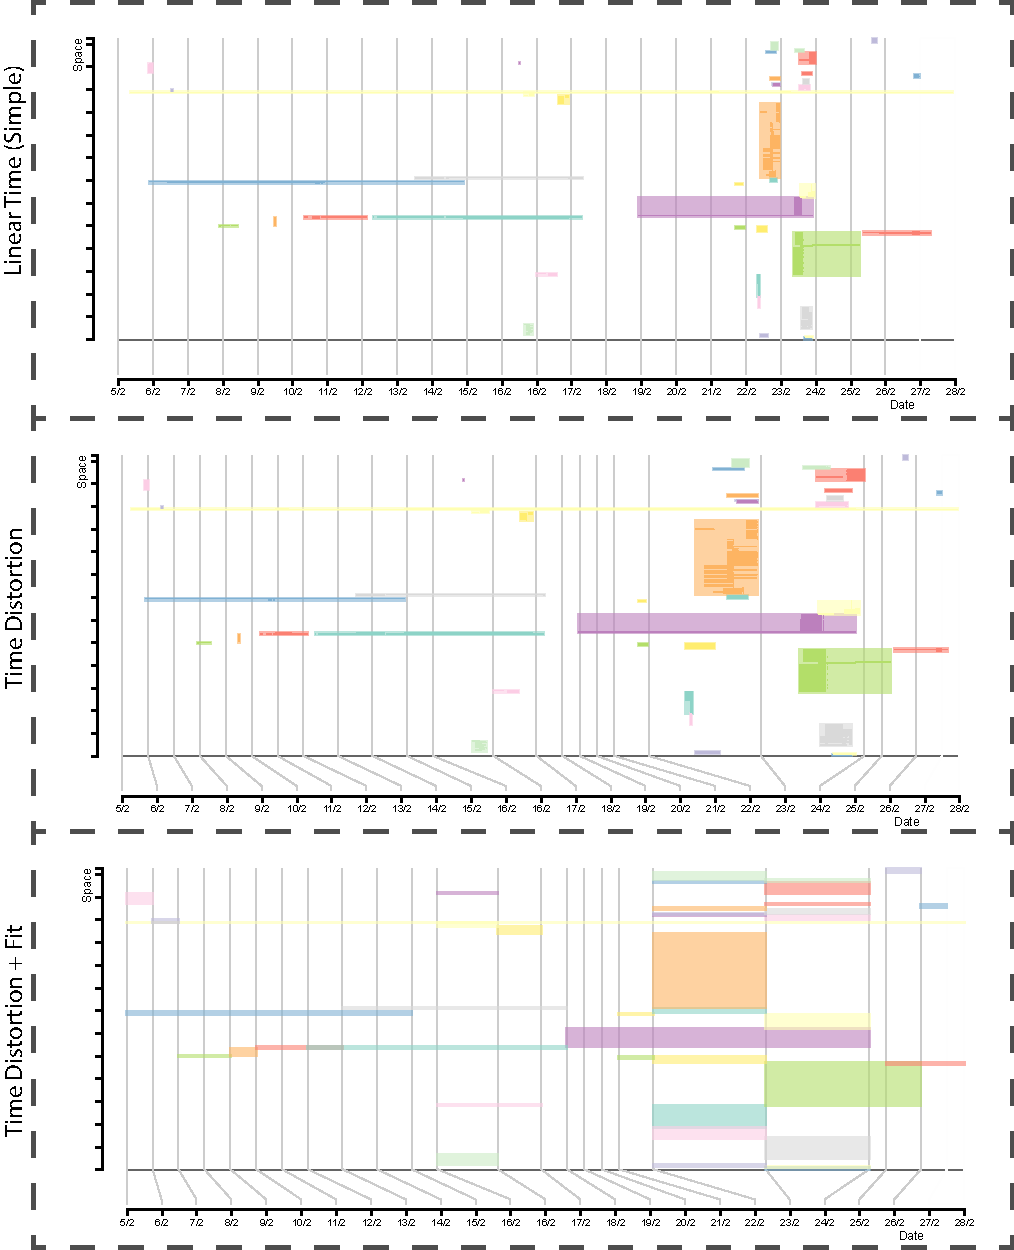
\includegraphics[width = 0.6\textwidth]{src/imgs/time-scale-explanation.pdf}
    \caption{Source: elaborated by author. Comparison of three different types of time scale used in example data from the use case.}
    \label{fig:time-scale-explanation}
\end{figure}

On the left of the plot, there is a color bar that indicates visually the quality of the spatial representation in the y-direction. 
%
This color bar is created by moving all the inner rectangles to the left of the figure, keeping the vertical positions.
%
The color of rectangles is based on a 2D color map from the original space of objects to the vertical position.
%
Each rectangle receives a color based on the center position of the respective point by placing this center position in a grid of size $512\times 512$, and picking the color of the respective pixel in the image of the color map.
%
It is exemplified in Figure~\ref{fig:colormap-example}, with some points in the center of the city of Rio de Janeiro and a respective color bar created.
%
As neighborhoods in the original space will receive similar colors, the continuity of the colors on the bar indicates good neighborhood preservation.

\begin{figure}
    \centering
    \includegraphics[width = 0.6\linewidth]{src/imgs/colormap-example.pdf}
    \caption{Source: elaborated by author. Example of the use of the color map to create a color bar.}
    \label{fig:colormap-example}
\end{figure}

To permit the analysis of different subsets of data and the interpretation of the results of the main plot, two methods for interactivity are implemented that link the Events-Vis view to the other two views.
%

A parallel coordinates plot positioned on the top right of the page is created to permit filtering the data. 
%
The plot contains vertical axes, each based on an attribute. 
%
For each point of data, in our case for each event, a line is placed connecting the positions of the respective values in each scale.
%
In Figure~\ref{fig:parallel-example}, the plot is created based on three attributes of the events: \textit{number of alerts, duration}, and \textit{area}.

\begin{figure}[hb]
    \centering
    \includegraphics[width = 0.7\linewidth]{src/imgs/parallel-coordinates.pdf}
    \caption{Source: elaborated by author. Example of a parallel coordinates with three attributes.}
    \label{fig:parallel-example}
\end{figure}

This permits the user to look for a general overview of the non spatio-temporal attributes,
%
and it is possible to make a selection in each of the axes, filtering the data based on thresholds of these attributes.
%
This filtered data is then pre-processed and the visualization in the main panel is updated, 
%
it permits to avoid cluttering
%
and to analyze spatio-temporal characteristics of objects with properties of particular interest.

On the bottom right of the page, there is a static map that contains a scatter plot of all objects of a particular time interval, a conventional method for the visualization of spatio-temporal data.
%
This data plot is used with selections in the Events-Vis plot, 
%
the users can click in a rectangle to highlight it on the map view.
%
In this map view, the user can look for the individual points by hovering, with a panel with attributes appearing.


\section{Evaluation}

Different variations of the visualization method were proposed, and it is necessary to evaluate if any of the adaptations considered increased the quality of the representation of the original data.
%
The variations are on the projection method used to obtain an ordering of events, and after that, the different methods for vertical positioning must also be compared.
%
The important criteria are the preservation of the distances between events (and between inner points), the preservation of the neighborhoods, and the quality of the representation of areas and intersections areas.
%
The computing time is also an important metric because, in an analytical scenario, fast queries are needed, and the method cannot take too long to generate a visualization.

\subsection{Metrics}

To evaluate the method, it will be used metrics that are common in the literature and also some particular for this work.
%
The first metric considered is the stress measure $S$, already presented in \ref{eq:stress-measure} for measuring the quality of distances preservation. It can be used with the center position of events or with the center position of the inner points.
%

%As our method only use the order of events obtained in the projection, the absolute value of positions is not a focus of representation, so we can use the stress-measure only considering the order of distances. 
%
%This change is also used in non-metric MDS.
%
%The change from stress-measure will be that $\overline d_{i, j}$ will substitute $d_{i, j}$ in the formula, 
%
%and will not be the distance between points $i$ and $j$, but the order of $d_{i,j}$ in the sequence of distances $\{d_{i, 1}, \dots, d_{i, n}\}$.
%

To measure the quality of the neighborhood preservation it was used the preservation of the $k$ nearest neighbors from the original space to the represented space.
%
Let $K_i$ and $K_i'$ be the set of $k$ nearest events to an event $e_i$ in the 2D space and the 1D result, respectively, i.e., let $\delta_k$ be the distance to the $k$-closest event of $e_i$, and $\Delta$ be the function that return the distance between two events, $K_i = \{ e_j |  \Delta(e_i, e_j ) \leq \delta_k, j \neq i \}$.
%
For each event $e_i$, we compute the size of the intersection set of $K_i$ and $K_i'$ and calculate the mean. 
%
We finally define it as: 
%
\begin{equation}
    error_N = \frac{1}{n}\sum_{i = 1}^n 1 - \frac{|K_i \cap K'_i|}{k}
\end{equation}

In particular to the proposed visualization, it was also measured the quality of the representation of intersections, it is the difference between the real and represented intersections. 
%
With  $\tilde{I}_{i, j}$ the intersection of the segments $(i, j)$ in the final plot, it is sum the absolute differences between it and $w_{i, j}$. We divide by  $\overline{w}$, the sum of all $w_{i, j}$, to normalize the error, so it will be proportional to the total size of intersections.

\begin{equation}
    error_I = \frac{1}{\overline{w}}\sum_{i =1}^n \sum_{j = i +1}^n |w_{i, j} - \tilde{I}_{i, j}|
\end{equation}

Two increase the detail in the metric, two versions were created, one version considers the error only when it is desired to have intersections and the other version considers the error when it should be no intersection, respectively, the \textit{non zero intersection error} and \textit{zero intersection error}:

\begin{equation}
    error_{I \geq 0} = \frac{1}{\overline{w}}\sum_{i =1}^n \sum_{j = i +1}^n |w_{i, j} - \tilde{I}_{i, j}| \mathbb{I}_{[w_{i, j} \geq 0]}
\end{equation}

\begin{equation}
    error_{I = 0} = \frac{1}{\overline{w}}\sum_{i =1}^n \sum_{j = i +1}^n |\tilde{I}_{i, j}| \mathbb{I}_{[w_{i, j} = 0]}
\end{equation}


\subsection{Evaluation-tool}
\label{sec:evaluation-tool}

\begin{figure}
    \centering
    \includegraphics[width = \textwidth]{src/imgs/evaluation-tool.pdf}
    \caption{Source: Elaborated by author. The interface of the tool for the evaluation of different methods with generated datasets created by the user.}
    \label{fig:evaluation-tool}
\end{figure}

To facilitate the comparison between the projection and vertical positioning methods it was also implemented a tool for the analysis of the results for different datasets.
%
Using the same languages and libraries as the visualization tool, this interface can be divided into three panels as shown in Figure~\ref{fig:evaluation-tool}: a) a menu for the selection of the computed methods and information with the metrics for the respective methods, b) a panel where the user can draw events shapes with mouse clicks and c) a plot with the resulted visualization.
%
Below, not visible on the figure, there is also a panel with the mathematical description of the optimization methods.

%
This application permits the user to draw any set of events as convex polygons with mouse clicks, so it facilitates understanding the results and verifying hypotheses, 
%
however, it is a simplified version of the method,
%
the events are polygons, but it is not possible to represent the inner structure,
and it ignores the time information of events, 
%
so the final plot will have rectangles positioned horizontally in an arbitrary order and with fixed width.

On the top panel Fig.~\ref{fig:evaluation-tool} a), the user can select as many methods as they desire, there are two buttons with symbols \textit{+} and \textit{-} that respectively add a new method and remove the last method add.
%
Each method is represented in a row of the table, with the columns being the parameters and error metrics of the method.
%
In order, the parameters are the projection method (PCA, MDS, t-SNE, UMAP, Hilbert, Morton), the optimization method (greedy, convex), if the height will be optimized and if the intersections equal to $0$ will be considered, two options only necessary for the convex method, and the values for parameters $(\lambda, \tau_1, \tau_2)$ if the height will be optimized.
%
So if the user wants to use the greedy algorithm, it can select only the projection method and the optimization method, leaving the other values as default.

In the same table, there are also columns for the metrics, that will only appear after the plot is created.
%
In order, the metrics are the \textit{intersection error}, \textit{non-zero intersection error}, \textit{zero intersection error}, \textit{stress measure}, \textit{neighborhood error}, and \textit{height error}.

Below this table there are the controls for data selection, first, there is a selector to choose between a set of pre-determined datasets, that will be plotted by clicking on \textit{Load}.
%
The button \textit{Reset} is to delete all events drawn in the plot, and the button \textit{Update} is to make the information for the server, which will compute the resulting visualization and the metrics.

In Fig.~\ref{fig:evaluation-tool} b) is the panel for a plot of events that is interactive. When hovering this panel, a purple circle will appear, by clicking, the circle will be fixed, being the first point of the event, the user can create as many points a desire by clicking. To finish an event, the user must hold the \textit{shift} key, the purple circle will get darker, when clicking, the event is sent to the server, which will return the convex hull of points to substitute the circles. 
%
An example of this process is presented in Figure~\ref{fig:evaluation-tool-draw}.

\begin{figure}
    \centering
    \includegraphics[width = 0.5\textwidth]{src/imgs/evaluation-tool-draw.pdf}
    \caption{Source: elaborated by author. An example process of creating a square event. On a) a purple circle is drawn under the cursor, on b) after a click, the first circle is fixed and another circle appears under the cursor, on c) three points are already fixed and when holding \textit{shift}, the circle under the cursor appears dark, on d) after clicking, the circles are substituted by the convex hull.}
    \label{fig:evaluation-tool-draw}
\end{figure}

After drawing a set of events, the user can click on \textit{Update} and it will be computed the vertical positioning algorithm, and the final plot will be shown in Fig.~\ref{fig:evaluation-tool-draw} c).
%
If there is more than one selected method, the plot will be divided in subplots of the same width, each subplot will have the result of a method. 
%
In the figure, three methods are selected, having three results.
%
The events are placed horizontally ordered by the y-position and with a fixed width to make them create small horizontal intersections just to be able to verify intersections.


\section{Data}

\begin{figure}
    \centering
    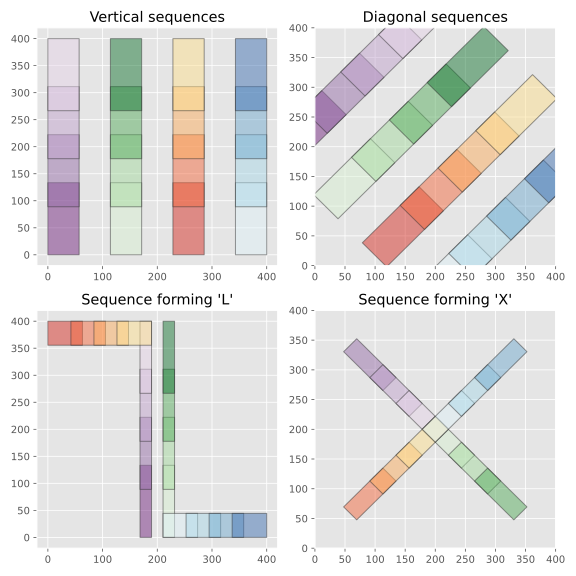
\includegraphics[width = \textwidth]{src/imgs/generated-datasets.pdf}
    \caption{Source: elaborated by author. Generated datasets, each rectangle represents an event, the colors are only indicative of "groups" of events. }
    \label{fig:generated-datasets}
\end{figure}
To evaluate the method and also demonstrate its applicability, it was made a selection of generated datasets and available spatio-temporal datasets.
%

\subsection{Generated datasets}

The intention of the generated datasets is to create simple patterns and verify the representation of this pattern in the generated visualization,
%
and also present examples that highlight the good properties of the presented method.
%
With that in mind, datasets shown in Fig.~\ref{fig:generated-datasets} were created by the repetition of simple shapes, rectangles whose center calculations are easy, areas, and intersection areas. The events created do not have a time attribute.
%

As shown in Figure~\ref{fig:generated-datasets}, it is possible to identify that are "columns" of events intersecting each other, these columns are also marked by color. 
%
These columns evaluate if the projections and the intersection adjustment will keep events from the same column together and if objects from different columns will intersect each other.
%
These datasets will be available to select on the evaluation tool previously presented.

\subsection{Real world dataset}

The real-world data is from the Waze app.
%
The data collected from the app are alerts created from users to notify accidents, roadwork, traffic changes from the city of Rio de Janeiro.
%
The available data is from a longer period of time, and different subsets can be created by selecting the time interval.
%
Each row of data contains information about: identification of the alert, date with hour and minutes, position (longitude, latitude), type, subtype, a comment explaining the alert, number of likes, reliability, and confidence of the alert.
%
There are many alerts each day, but much of the data is a repetition of the same alert with different timestamps. 
%
It was used two subsets of the data, in both cases only considering alerts where the user add a commentary explaining it, the first subset is from the interval of 1/12/18 to 31/03/19, the second is only from the month of February of 2019.
%
The first one is going to be present in the use-case~\ref{sec:use-case}, and the second is used on the examples figures in the Section~\ref{sec:visualization-tool}.
%
A general overview of the datasets is available at Figs.~\ref{fig:waze-overview}.

\begin{figure}
    \centering
    \includegraphics[width = \textwidth]{src/imgs/waze-datasets.pdf}
    \caption{Source: elaborated by author. General characteristics from Waze dataset on both subsets, with spatial distribution, temporal histogram, and distribution by type and subtype of alerts.}
    \label{fig:waze-overview}
\end{figure}


To transform this dataset into events it is necessary to apply a clustering algorithm,
%
each cluster of points from a specific spatial region in a time interval can be generated by an urban event in the city, 
%
such as an accident, the carnival festivities, roadwork.
%
The clustering algorithm will be the ST-DBSCAN presented in section \ref{sec:clustering} with small changes.

%
The initial change is that the parameter $\Delta \varepsilon$ is not used. 
%  
Another adaptation is to consider points with temporal duration. Let $p \in D$, it is defined the points $p_{t0}$ and $p_{t1}$ with same spatial position and different temporal values, $p$ is the segment that connects $p_{t0}$ and $p_{t1}$. The temporal neighborhood of $p$ is the interval $[p_{t0} - Eps_2, p_{t1} + Eps_2]$. The neighborhood is exemplified in Figure \ref{fig:stdbscan_neighborhood}.

\begin{figure}
    \centering
    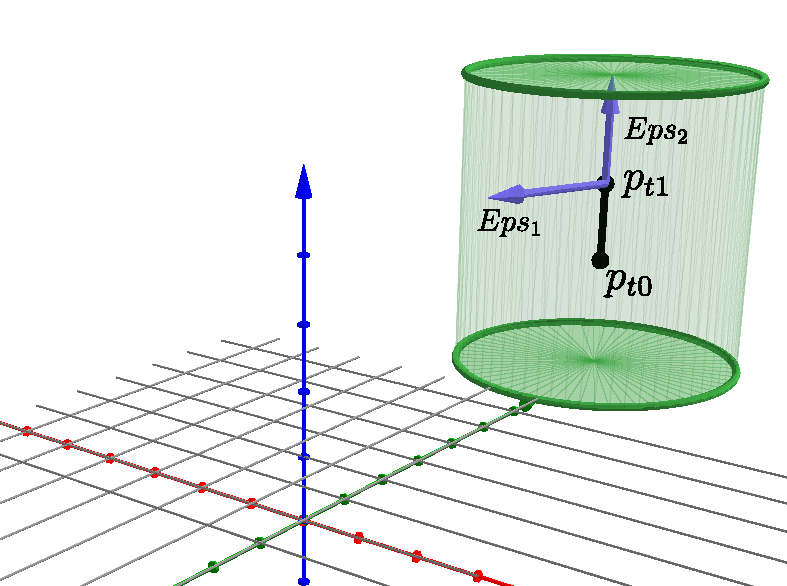
\includegraphics[width = 8cm]{src/imgs/point_neighborhood_stdbscan.pdf}
    \caption{Source: Elaborated by author. Example of point neighborhood, the point is actually a segment perpendicular to the plane $XY$, from points $p_{t0}$ to $p_{t1}$, the green cylinder is the neighborhood, the form is because of the quadratic distance in the spatial dimension and the linear distance in time.} 
    \label{fig:stdbscan_neighborhood}
\end{figure}

 
%
The last adaptation is the use of another attribute called \textit{subtype}, points will be in the same neighborhood if their values for \textit{subtypes} are equal. 

%
To compute spatial neighborhoods it will be used the euclidean distance, for that it is necessary to project the coordinates to the UTM system,
%
because in small regions it is a good approximation of a planet's surface and the distances can be computed with the euclidean formula.
%
The neighborhood size parameters used in the examples are selected by testing, with a set of parameters values, in each one it was computed the clustering and the result was analyzed with the visualization tool~\ref{sec:visualization-tool}, verifying if the points from the same cluster are coherent.

%
%The algorithm for retrieving neighbors considering the implement changes is at \ref{alg:retrieve_neighbors}.

%\begin{algorithm}[H]
%\label{alg:retrieve_neighbors}
%\SetAlgoLined
%\SetKwInOut{Input}{Input}
%\Input{
%$p$ - point with attributes \\
%$Eps_1$ - threshold for spatial distance in neighborhood \\
%$Eps_2$ - threshold for temporal distance in neighborhood \\
%}
%\SetKwInOut{Output}{Output}
%\Output{
%$N$ - subset of points in the neighborhood
%}
%\tcc{find all points from $D$ that are inside the circle of center $p$ and radium $Eps_1$} 
%$N = $ kdtree\_query$(p, Eps_1)$\;
%\tcc{find all points from $N$ that are inside the segment of %temporal neighborhood}
%$N = $ temporal\_query$(p, N, Eps_2)$\;
%\tcc{find all points from $N$ of same subtypes}
%$N = $ subtype\_query$(p, N)$\;
%\caption{Algorithm for retrieving neighbors of point $p$ in the %ST-DBSCAN algorithm.}
%\end{algorithm}




\chapter{Results}
\label{ch:results}

The results of this work will be presented in the visual analysis of the result of the visualizations and in numerical evaluations.
%
It is necessary to compare the different projections methods and the different methods for vertical positioning,
%
and the used datasets are the generated ones from previous sections and the traffic data.

\section{Projections comparisons}

In Figures~\ref{fig:generated-datasets-dimensionality-reduction}~and~\ref{fig:generated-datasets-spatial-indexing} are shown the results of the projection method applied to the generated datasets (vertical, diagonal, 'L', 'X'), all events are shown with the same size and with the same vertical position, the object is just to verify the ordering.
%
The characteristics that are going to be looked are: if objects of the same sequence (color) are projects together, if the objects of the same sequence (color) are projected with sequential coherence (gradual change in color) and if the different sequences are projected in a coherent manner.
For this comparison, we are using the greedy vertical positioning method.

Starting on the analysis of Fig.~\ref{fig:generated-datasets-dimensionality-reduction}, we will look at each dataset and compare the visual representation of the dimensionality reduction methods.
%

\begin{figure}
    \centering
    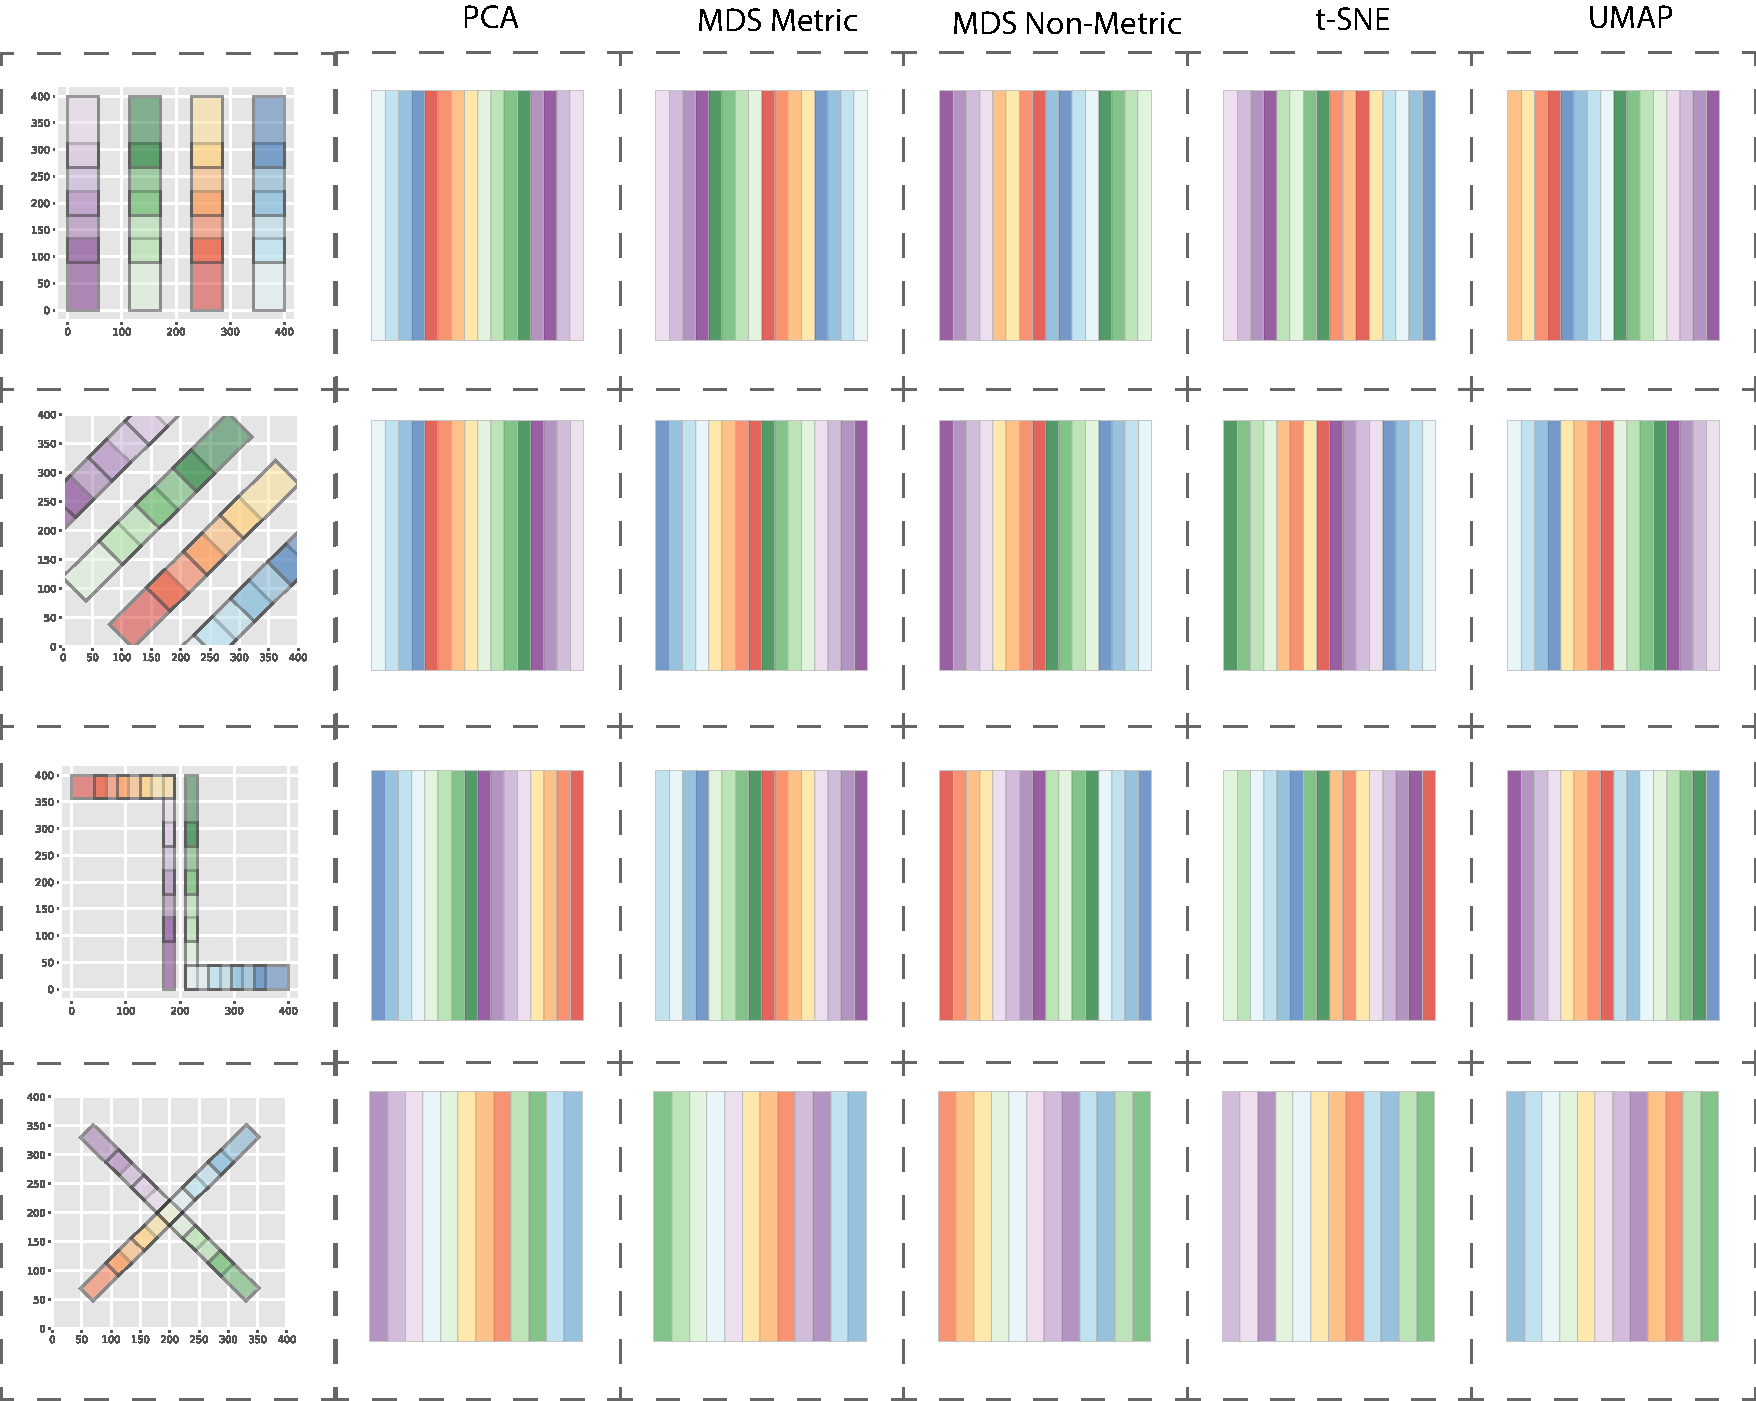
\includegraphics[width = \textwidth]{src/imgs/generated-datasets-dimensionality-reduction.pdf}
    \caption{Source: elaborated by author. Ordering of events using the generated datasets and different dimensionality reduction methods. The events are placed horizontally based on the projection ordering.}
    \label{fig:generated-datasets-dimensionality-reduction}
\end{figure}


\begin{itemize}
    \item \textit{Vertical} dataset: all projection methods kept the events from the same sequence (column) together, with mostly gradual changes in color. However, PCA, MDS-Metric, and t-SNE were able to keep the horizontal order of columns: purple, green, orange, blue (or the inverse). MDS-Metric contained the most gradual smooth inside each sequence.
    \item \textit{Diagonal} dataset: both PCA, MDS and UMAP had a good quality of representation, but the t-SNE mixed the order of diagonals. The result of UMAP was better than the previous.
    \item \textit{"L"} dataset: the PCA represented the order of columns based on the horizontal order. MDS-Metric and Non-Metric created discontinuities inside the sequences. UMAP and t-SNE mixed sequences.
    \item \textit{"X"} dataset: is the hardest to represent in 1-dimension due to the mix of the colors in the center.
    The most common representation was to show objects of the center and after the darker colors outer events, PCA, MDS-Metric and MDS Non-Metric showed this results.
    With t-SNE there was a mix between dark and lighter colors, and UMAP mixed some blue events and a dark red event.
\end{itemize}

Now analyzing Figure~\ref{fig:generated-datasets-spatial-indexing}, we analyze the results with spatial indexing methods and compare the different orders of the space-filling curve. Looking at each dataset:

\begin{figure}
    \centering
    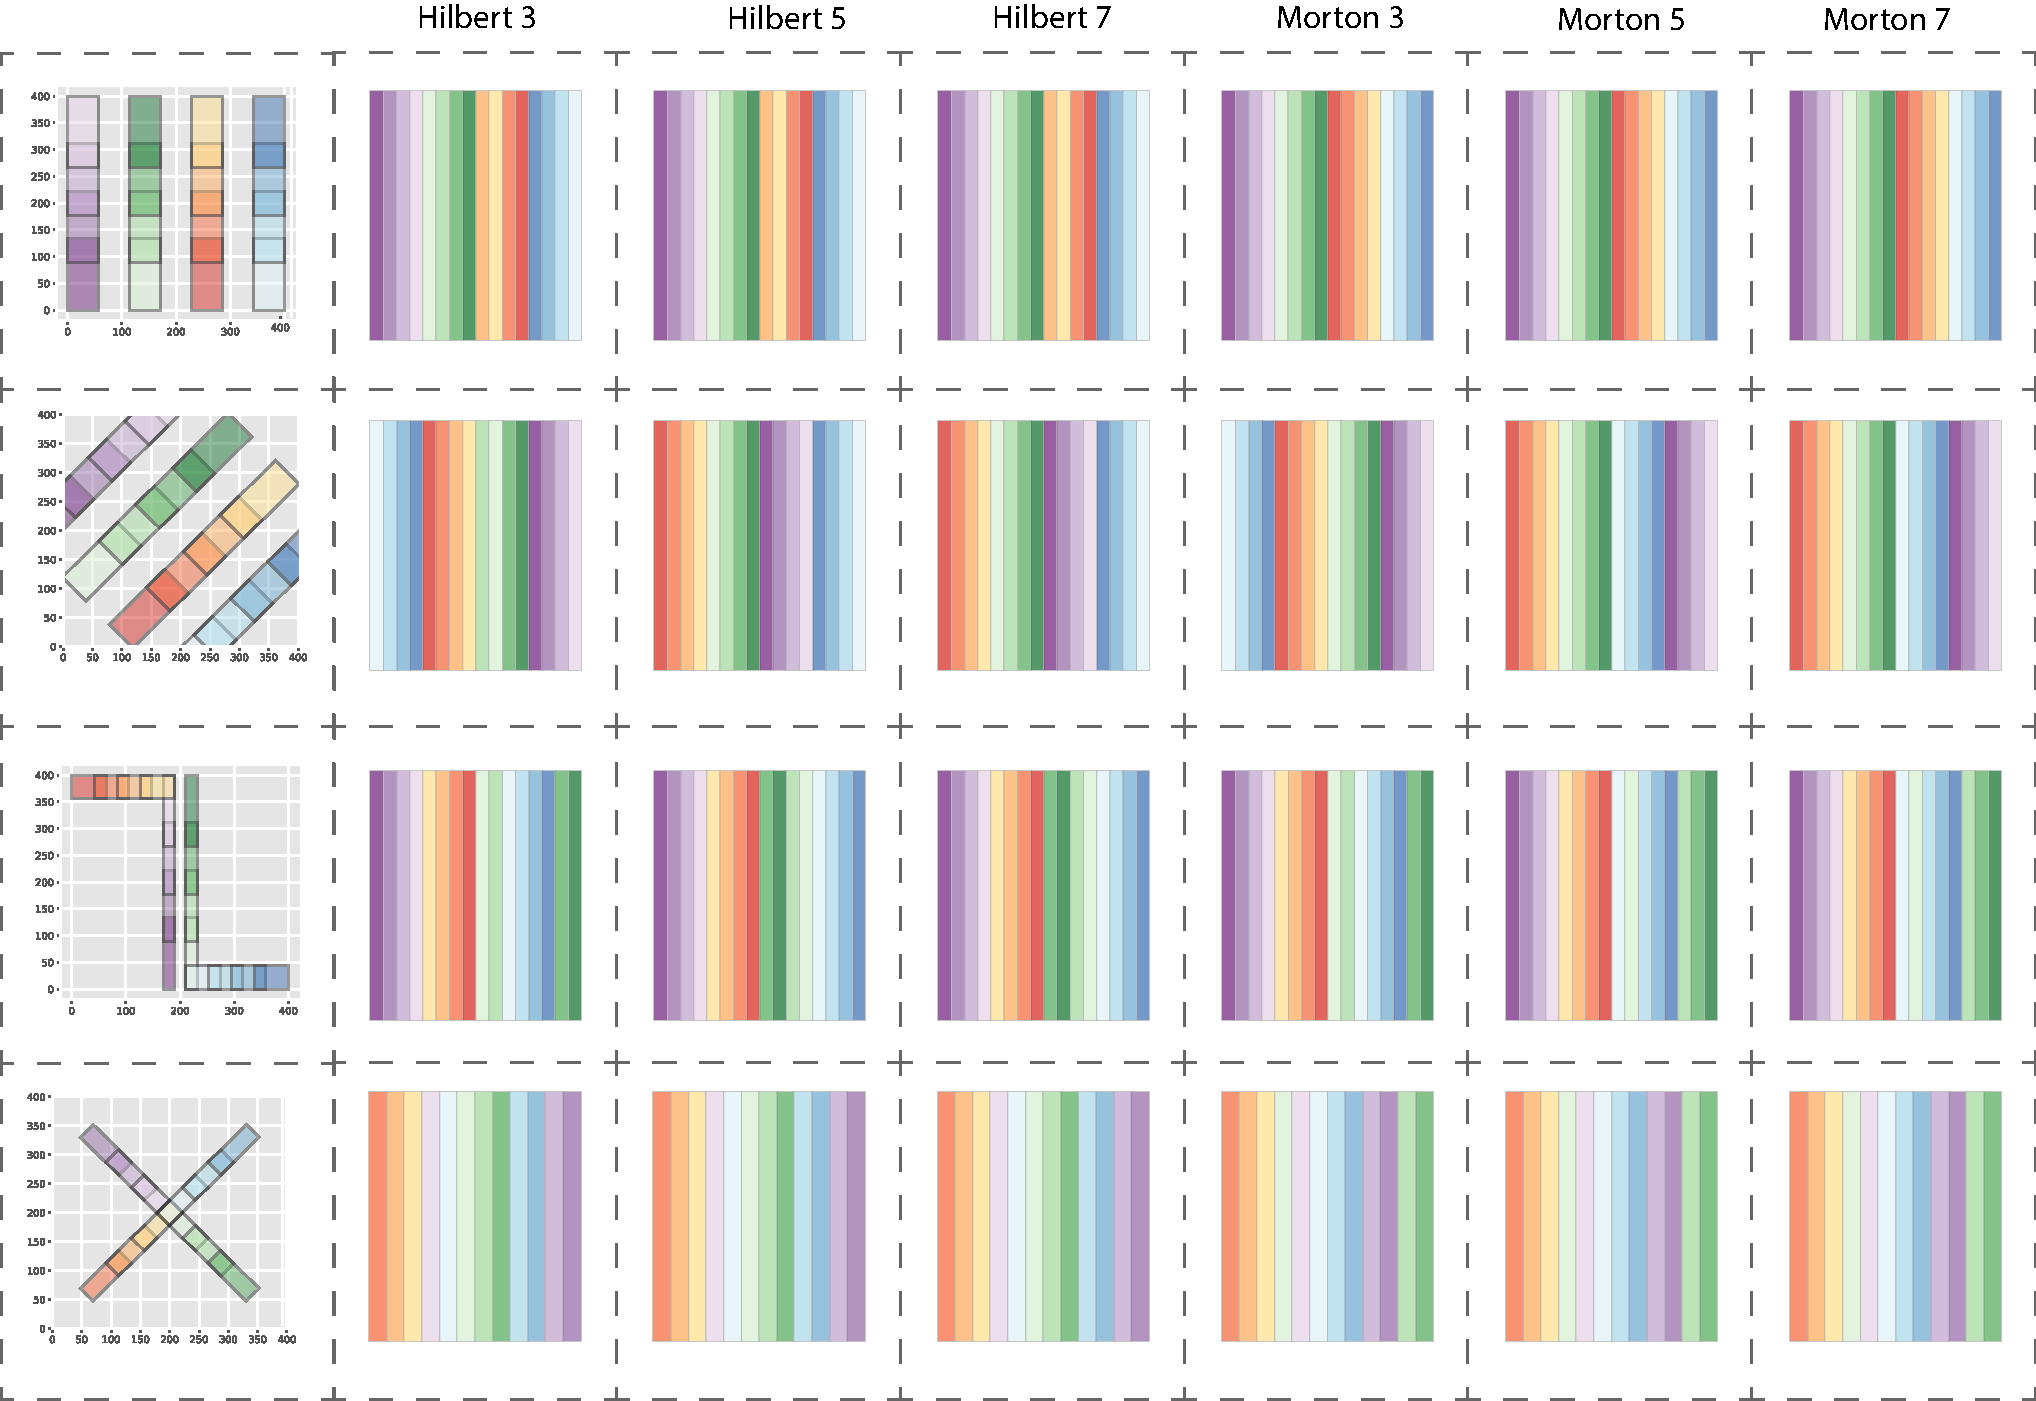
\includegraphics[width = \textwidth]{src/imgs/generated-datasets-spatial-indexing.pdf}
    \caption{Source: elaborated by author. Ordering of events using the generated datasets and different spatial indexing methods. The events are placed horizontally based on the projection ordering.}
    \label{fig:generated-datasets-spatial-indexing}
\end{figure}

\begin{itemize}
    \item \textit{Vertical} dataset: All methods were able to preserve the different columns of events, and all results were the same independently of the order of the curve. Hilbert presented discontinuities on the red sequence, while Morton ordered it gradually.
    \item \textit{Diagonal} dataset: It is possible to view changes from the curve of order 3 to order 5, although the events are making jumps from the color blue to the color purple in the curves or order 5 and 7, opposite sides of the space.
    \item \textit{"L"} dataset:  The ordering is again pretty similar in all curves, with changes from order 3 to order 5 on the Hilbert curve. In all cases, the sequences were not placed following a direction.
    \item \textit{"X"} dataset: the hardest dataset for dimensionality reductions method, showed similar results with spatial-indexing. All curves started with red events, exhibited events of light  color. The dark colors were placed gradually.
\end{itemize}





We also analyze the numeric error values for the different projection methods.
%
The numeric results confirm our previous commentaries, it is possible to identify the best results considering the stress measure on all datasets is with the use of the PCA.
%
The space-filling curves were the second best, with really similar values to PCA, with the exception of the \textit{Rotated} dataset, where they were the worst projection method.
%

Regarding the neighborhood error, the results were similar in all projections with all datasets. One special case is the \textit{L} dataset where the curves Hilbert of orders 5 and 7 had a smaller value than the other space-filling curves.
%
Looking now at the processing time, the use of the UMAP projection method is the only one that passed on second, presenting no advantage in comparison with the other methods.

\begin{table}[tb]
\centering
\resizebox{0.4\linewidth}{!}{%
\begin{tabular}{
    c |
	S[table-number-alignment = center]
	S[table-number-alignment = center]
	S[table-number-alignment = center]
	}
\hline
{Projection method} & {$S$} & {$N$} & {time (s)} \\ \hline
\multicolumn{4}{c}{\textit{Vertical} dataset}  \\ \hline
PCA	& 0.37 & 0.52 & 0.03 \\
MDS Metric	& 0.59	& 0.5	& 0.04 \\
MDS Non-Metric	& 0.6	& 0.52	& 0.05 \\
t-SNE & 0.67	& 0.58	& 0.88 \\
UMAP	& 0.59	& 0.5	& 5.7 \\
Hilbert order 3	& 0.36	& 0.5	 & 0.02 \\
Hilbert order 5	& 0.36	& 0.5		& 0.03 \\
Hilbert order 7 & 0.36	& 0.5		& 0.03 \\
Morton order 3 & 0.36	& 0.5		& 0.03 \\ 
Morton order 5	& 0.36	& 0.5		& 0.03 \\
Morton order 7 & 0.36	& 0.5		& 0.02 \\ \hline
\multicolumn{4}{c}{\textit{Rotated} dataset}  \\ \hline
PCA	& 0.36	& 0.5		& 0.05 \\
MDS Metric	& 0.36	& 0.5		& 0.07 \\
MDS Non-Metric	& 0.59	& 0.5		& 0.08 \\
t-SNE	& 0.51	& 0.54		& 0.96 \\
UMAP	& 0.37	& 0.48	&	5.62 \\
Hilbert order 3	& 0.36	& 0.54		& 0.02 \\
Hilbert order 5	& 0.59	& 0.5		& 0.03 \\
Hilbert order 7 & 0.59	& 0.5		& 0.04 \\
Morton order 3	& 0.36	& 0.5		& 0.03 \\
Morton order 5	& 0.59	& 0.5		& 0.02 \\
Morton order 7	& 0.59	& 0.5		& 0.03 \\
\end{tabular}
%
}
\quad
\resizebox{0.4\linewidth}{!}{%
\begin{tabular}{
    c |
	S[table-number-alignment = center]
	S[table-number-alignment = center]
	S[table-number-alignment = center]
	}
\hline
{Projection method} & {$S$} & {$N$} & {time (s)} \\ \hline
\multicolumn{4}{c}{\textit{"L"} dataset}  \\ \hline
PCA & 0.31	& 0.29		& 0.05 \\
MDS Metric	& 0.55	& 0.31		& 0.06 \\
MDS Non-Metric	& 0.31	& 0.29		& 0.12 \\
t-SNE	& 0.63	& 0.46		& 0.75 \\
UMAP	& 0.55	& 0.42	&	5.48 \\
Hilbert order 3	& 0.67	& 0.44		& 0.03 \\
Hilbert order 5	& 0.55	& 0.33	& 	0. 02 \\
Hilbert order 7	& 0.55	& 0.33		& 0.03 \\
Morton order 3	& 0.67	& 0.44		& 0.03 \\
Morton order 5	& 0.7	& 0.4		& 0.02 \\
Morton order 7	& 0.7	& 0.4		& 0.03 \\
 \hline
\multicolumn{4}{c}{\textit{"X"} dataset}  \\ \hline
PCA	& 0.48	& 0.33		& 0.02 \\
MDS Metric	& 0.48	& 0.39		& 0.03 \\
MDS Non-Metric	& 0.63	& 0.56		& 0.04 \\
t-SNE & 0.49	& 0.31		& 0.81 \\
UMAP	& 0.63	& 0.53	&	5.49  \\
Hilbert order 3	& 0.48	& 0.31		& 0.03  \\
Hilbert order 5 & 0.48	& 0.31		& 0.02  \\
Hilbert order 7	& 0.48	& 0.31		& 0.02  \\
Morton order 3	& 0.52	& 0.33		& 0.02 \\
Morton order 5	& 0.52	& 0.33		& 0.02 \\
Morton order 7	& 0.52	& 0.33 	& 0.02 \\

\end{tabular}
%
}
\caption{Metric results and computation time for projection methods comparison on generated datasets.}
\label{table:1}
\vspace{-0.5cm}
\end{table}

With the results presented, it is concluded that the best methods for projection are the PCA and the space-filling curves, with no dominant curve order.

\section{Vertical positioning comparison}

We now look at the different versions of the vertical positioning step in the Events-Vis technique.
%
In this section, we made use of the generated datasets but also the evaluation-tool~\ref{sec:evaluation-tool} for the liberty of drawing different situations of events.
%
The section is organized based on questions that will be answered with examples. 

\textbf{Q1: The simple convex optimization is able to surpass the results from the greedy method?}

In most of the simple cases, the result of the greedy and the convex optimization methods are the same. In Figure~\ref{fig:vert-pos-alg1} A1 and A2, both results are identical using the greedy and the simple convex optimization method. In particular, in example A1 the intersection error was equal to 0.
%
Using the evaluation-tool interface, it is hard to draw a situation where the greedy is worse than the convex optimization, and no pattern of pitfalls of the greedy was identified.

\textbf{Q2: What is difference in the results of the convex optimization opting for the optimization in the cases where $w_{i, j} = 0$ and to ignore it?}

This question is answered in Fig.~\ref{fig:vert-pos-alg1} B1 and B2, some problems of ignoring to optimize the pairs of events with no intersection, is that it can be advantageous for the method to place two events in the same position when in reality they do not intersect, as occurs in B1.
%
However, in some cases, they can also present better results, as shown in B2.
%
The advantage of ignoring zeros is that the problem becomes easier, depending on a smaller number of decision variables, and the optimizing time can be really smaller than when the zeros are optimized.

\begin{figure}
    \centering
    \includegraphics[width = \linewidth]{src/imgs/vert-pos-alg1.pdf}
    \caption{Source: elaborated by author. Examples for questions Q1 and Q2. The circles on B1 and B2 indicates good (green) and bad (red) representations of intersections.}
    \label{fig:vert-pos-alg1}
\end{figure}

\textbf{Q3: When optimizing the heights of rectangles in the convex optimization method, what is the effect of varying the parameters $(\lambda, \tau_1, \tau_2)$?}

In most cases, the result with any combination of parameters is the same if the height was not optimized.
%
We can interpret this that the best solution is always to keep the heights, even when then the parameter $\lambda$ is small and the error in height is not penalized.
%
In Fig.~\ref{fig:vert-pos-alg2} C1 is shown an example and the same result for a different set of parameters.

\textbf{Q4: What is the processing time of the different methods?}

With really simple examples, as many of the present above, all the methods are able to solve in less than a second, not showing an important difference in time.
%
However, when the problem increase in size, i.e., the number of events increases the optimization method starts to take a long time.
%
We can compose the \textit{vertical} and \textit{rotated} datasets as shown in Figure~\ref{fig:vert-pos-alg2} D1, creating a big subset of intersections.
In that case, the greedy method is able to solve in $0.1$ seconds, the convex optimization simple in $8.81$ seconds, and if we select to ignore the zeros, the time decrease to $1.63$ seconds. In particular, the intersection error in that scenario are respective $(0.13, 0.14, 0.18)$, so the increased processing time do not result in a better solution.

\textbf{Q5: Does the projection method impact the result of the method?}

The projection has a huge impact on the result of the intersection algorithm because of the restriction to keep the order of objects that is used both in the greedy and in the convex optimization method.
%
In Figure~\ref{fig:vert-pos-alg2}, it is presents two examples E1 and E2 using the simple convex optimization method with different projections, it is possible to see that depending on the ordering obtained, the intersections can be represented or not.

\begin{figure}
    \centering
    \includegraphics[width = \linewidth]{src/imgs/vert-pos-alg2.pdf}
    \caption{Source: elaborated by the author. Examples for questions Q3, Q4, and Q5. The circles and lines on E1 and E2 indicates good (green) and bad (red) representations of intersections.}
    \label{fig:vert-pos-alg2}
\end{figure}


\section{Use Case: Traffic on Rio de Janeiro}
\label{sec:use-case}

Rio de Janeiro is the center of significant events, as the New Year celebrations at Copacabana beach or the Carnival in the city center. 
%
Moreover, it is a city with a very high population density where there is a significant movement of people and vehicles affected by daily events. 
%
This study case use traffic alerts notified by Waze users collected from December 2018 until April 2019, containing a total of 9,648 alerts.

We used the Hilbert curve to project the events.
%
For the vertical positioning, we used the convex optimization method. 
%
Fig.~\ref{fig:waze-use-case} shows our result; at first glance, the vertical distribution of rectangles shows a good representation of the 2D space.
%
Note that we added some wiggle icons in the vertical axis to indicate the spatial distance between subsets of events. 
%
We also annotated the spatial regions (i.e., north, center, and south) to know where the majority of the events are located in the interval.

Analyzing this visualization, we can see some interesting patterns (see black rectangles). 
%
(i) The two events in region A1 correspond to the New Year celebration. 
%
In A2, we see that they are from two nearby beaches (Ipanema and Copacabana); our representation could preserve this fact in the vertical positioning. 
%
Moreover, they are events that inner points have the same width, i.e.,  temporal duration, except for one longer.
%
(ii) In B1, we can see a set of events with vertical overlap; to confirm that, we selected those events and generated the map on B2. 
%
Note that these events are in the city center during the carnival period and an event from a marathon.
%
(iii) In C1, we have two events with considerable vertical overlap. 
%
Our representation indicates that the events were in the same spatial region (we can confirm it in C2). 
%
Reading the alert descriptions, we note that they refer to two Carnival blocks on different days. 
%
Although the event in purple appears to have a longer duration, this is because a single internal alert lasted for several weeks. 
%
Finally, (iv) in D1, we see an event that is very small spatially but with a long duration.
%
Analyzing the alerts, we observe that the clustering algorithm put together notifications from Carnival blocks with reports from roadwork. 
%
This is because they were alerts in a near spatial and temporal location. 
%
Usually, roadwork alerts are the longest; they lasted more than a month in this specific case. 

\begin{figure}
    \centering
    \includegraphics[width = \linewidth]{src/imgs/waze-use-case.pdf}
    \caption{Source: elaborated by author. Events-Vis result with Waze app data from Rio de Janeiro.}
    \label{fig:waze-use-case}
\end{figure}

In summary, we can see how our representation of spatio-temporal events in a static visualization successfully fulfills its purpose. 
%
Analyzing this visualization, we have a global overview of the most predominant events in Rio de Janeiro during five months. 


\section{Discussion}
As earlier mentioned, the increase in the number of available spatiotemporal data motivates the development of different methods of analysis, including the use the visualizations.
%
This data can be in different types, geo-referenced time series, trajectories, events.
%
We presented a method for the visualization of events that is able to represent the general spatial and temporal distribution of them.
%
However, this restriction of the data type is a limitation to impede the use in many of the common datasets, for example, taxi trips, hurricanes trajectories.

The use of the ST-DBSCAN was also a difficulty of the technique in the generation of the events in the use case dataset.
%
It was necessary the test with many combinations of parameters of neighborhood size and minimum number of neighbors to identify a clustering with good interpretability.
%
On the other hand, it shows that our visualization is really helpful in the analysis of clustering.
%
In a scenario of the decision of parameters of a clustering method, the different combinations could be evaluated with the results obtained on the plot.

Different projections methods were considered to make a selection of the most adequate for the technique, and the result was that advanced techniques such as t-SNE and UMAP presented poor results.
%
This can be caused due to the hyper-parameters of the transformations, and the necessity to apply a fine-tuning to identify the best values for the used data.
%
This can be a consideration in future work, and after that, tricks could be used to give more information for the methods, for example, the extraction of a feature based on the area of intersection between events, so intersecting events could already be projected in close positions.  

On the vertical positioning step, the convex optimization method used was not able to surpass the results from the greedy heuristic, also presenting a problem of high processing time.
%
On future works, there is the interest in developing new methods for optimizing the representation of intersections, one possibility could relax the constraint of order of events, or even more, do not use the projection step and just apply an optimization.


\newpage 
\chapter{Conclusion}

In this work was presented an overview of different methods for spatiotemporal visualization and methods used space transformation.
%
Next, we propose Events-Vis, a method for visualizing spatio-temporal in a static visualization. 
%
This technique represents the space information in 1D preserving the neighborhoods and regions' intersection. 
%
We evaluate our technique using two metrics and multiple configurations. 
%
We also present a use case with real data from traffic in Rio de Janeiro. 
%
These results show the usefulness of Events-Vis to have a global view of spatio-temporal events using static visualizations. 


However, there is space for improvements. 
%
For instance, we want to consider other optimization methods in the positioning stage, for example, relaxing the constraint to keep the order of events.
%
Finally, we want to test our technique using other real datasets.




% ----------------------------------------------------------
% Referências bibliográficas
% ----------------------------------------------------------
\citeoption{abnt-etal-list=5}
\bibliographystyle{abntex2-cite-min}
\bibliography{references}



% ----------------------------------------------------------
% Glossário
% ----------------------------------------------------------
%
% Consulte o manual da classe abntex2 para orientações sobre o glossário.
%
%\glossary

% ----------------------------------------------------------
% Apêndices
% ----------------------------------------------------------

% ---
% Inicia os apêndices
% ---
%\begin{apendicesenv}

% Imprime uma página indicando o início dos apêndices
%\partapendices

% ----------------------------------------------------------
%\chapter{People who have worn the ring}
% ----------------------------------------------------------
%We have known some people that have worn the ring in the past. They are described in Table \ref{tab:ring_and_age}

\begin{table}[hb]
\centering
\begin{tabular}{cc}
\hline
Name    & Age       \\ \hline
Frodo   & 51        \\
Boromir & 41        \\
Smeagol & $\sim$600 \\ \hline
\end{tabular}
\caption{The age (in years) of people that have worn the ring}
\label{tab:ring_and_age}
\end{table}

% ----------------------------------------------------------
%\chapter{Nullam elementum urna vel imperdiet sodales elit ipsum pharetra ligula
%ac pretium ante justo a nulla curabitur tristique arcu eu metus}
% ----------------------------------------------------------
%\lipsum[55-57]

%\end{apendicesenv}
% ---


% ----------------------------------------------------------
% Anexos
% ----------------------------------------------------------

% ---
% Inicia os anexos
% ---
%\begin{anexosenv}

% Imprime uma página indicando o início dos anexos
%\partanexos


%\end{anexosenv}

%---------------------------------------------------------------------
% INDICE REMISSIVO
%---------------------------------------------------------------------
\phantompart
\printindex
%---------------------------------------------------------------------

\end{document}
